\section{Background Estimation}
\label{sec:analysis:background}


The \BWl measurement has four sources of standard model backgrounds:

\begin{itemize}
    \item vector boson plus jets (\wjets in counting analysis, \zjets)
    \item photon plus jets (\gjets)
    \item diboson production ($\PW\PW$ in counting analysis, $\PZ\PZ$, $\PZ\PW$)
    \item multijet QCD
\end{itemize}

It is worth pointing out that the \wjets and $\PW\PW$ processes are treated as backgrounds in counting analysis, but the shape analysis treats them as signals. This is because the counting analysis uses only the \ttbar enriched signal region, while the shape analysis includes extra control regions with relaxed jet multiplicities requirement. Overall, vector boson plus jets are the most prominent source of backgrounds. The contributions from \gjets are much smaller and mainly in the \ceh channel. The contributions from diboson processes $\PW\PW$, $\PZ\PZ$, $\PZ\PW$ are even smaller. In the \ttbar regions, the contributions from these backgrounds are very small in comparison with the signals. The backgrounds from \zjets, \wjets, \gjets and diboson processes are all well modeled by the simulated datasets. Non-negligible contamination from QCD processes are found in \cet, \cmt, \ceh, \cmh channels. The \HT-binned QCD simulations are evaluated, and turn out to be statistically sufficient at an acceptable level for the normalization in the $\ceh$ and $\cmh$ channels which requires high jet multiplicities $n_j\geq 4$. However, the number of simulated QCD events is insufficient for accurately modelling shape of kinematics distributions. Therefore, data-driven approaches are employed to estimate the QCD background in the \cet, \cmt, \ceh, \cmh channels. For \cet, \cmt channel, a same-sign region is used. For \ceh, \cmh channel, the region with inverted lepton isolation is used.



\subsection{QCD background in the $e \tau_\mathrm{h}$ and $\mu \tau_\mathrm{h}$ channels}

This estimation relies on the dearth of standard model processes that can give rise to same-sign lepton pairs.  It is expected that most events with same-sign lepton pairs are the result of at least one of the leptons coming from non-prompt decays.  It is further assumed that this process will give rise to misidentifying hadronic jets as leptons in near equal measure between the same sign and opposite sign selections.  

The process of deriving the estimate is simple enough: requiring the electron or muon having the same sign as the hadronic tau in the \cet and \cmt channel. All other selection requirements are kept unchanged. The deficit between data and standard model simulation in the same-sign side-band region is multiplied by a transferring scale factor to estimate the QCD contamination in the signal region. 


The same-sign (SS) to opposite-sign (OS) transfer scale factor transfer factor is calculated by
\begin{equation}
    SF^{\rm SS \to OS} = \frac{N^{\rm OS}_{\rm data} - \sum N^{\rm OS}_{\rm MC} }{ N^{\rm SS}_{\rm data} - \sum N^{\rm SS}_{\rm MC} }
\end{equation}
\noindent To determine $SF^{\rm SS \to OS}$, the counting analysis uses \cet and \cmt channels with $n_j=2,n_\PQb=0$. The SS and OS regions of \cet and \cmt channels with different $n_j,n_\PQb$ configurations are shown in Figure~\ref{fig:background:ltau:mass_ltau_1} and \ref{fig:background:ltau:mass_ltau_2}. The $SF^{\rm SS \to OS}$ measured from $n_j=2,n_\PQb=0$ is chosen because the jet and \PQb tag configuration is closest to the signal region. The corresponding results of $SF^{\rm SS \to OS}$ are 1.062 and 1.195 for \cet and \cmt channel, respectively.



For shape analysis, this region is treated as a signal region. So the regions with anti-isolated electron or muon plus \PGth with $n_j=0$ are used to measure  $SF^{\rm SS \to OS}$. Figure~\ref{fig:background:ltau:mass_ltau_antiiso} shows the $m_{\cet}$ and $m_{\cmt}$ distributions distributions in the same-sign and opposite-sign regions of \cet (on the right) and \cmt (on the left) channel with the anti-isolated lepton and zero jets.

\begin{figure}[h]
    \centering
    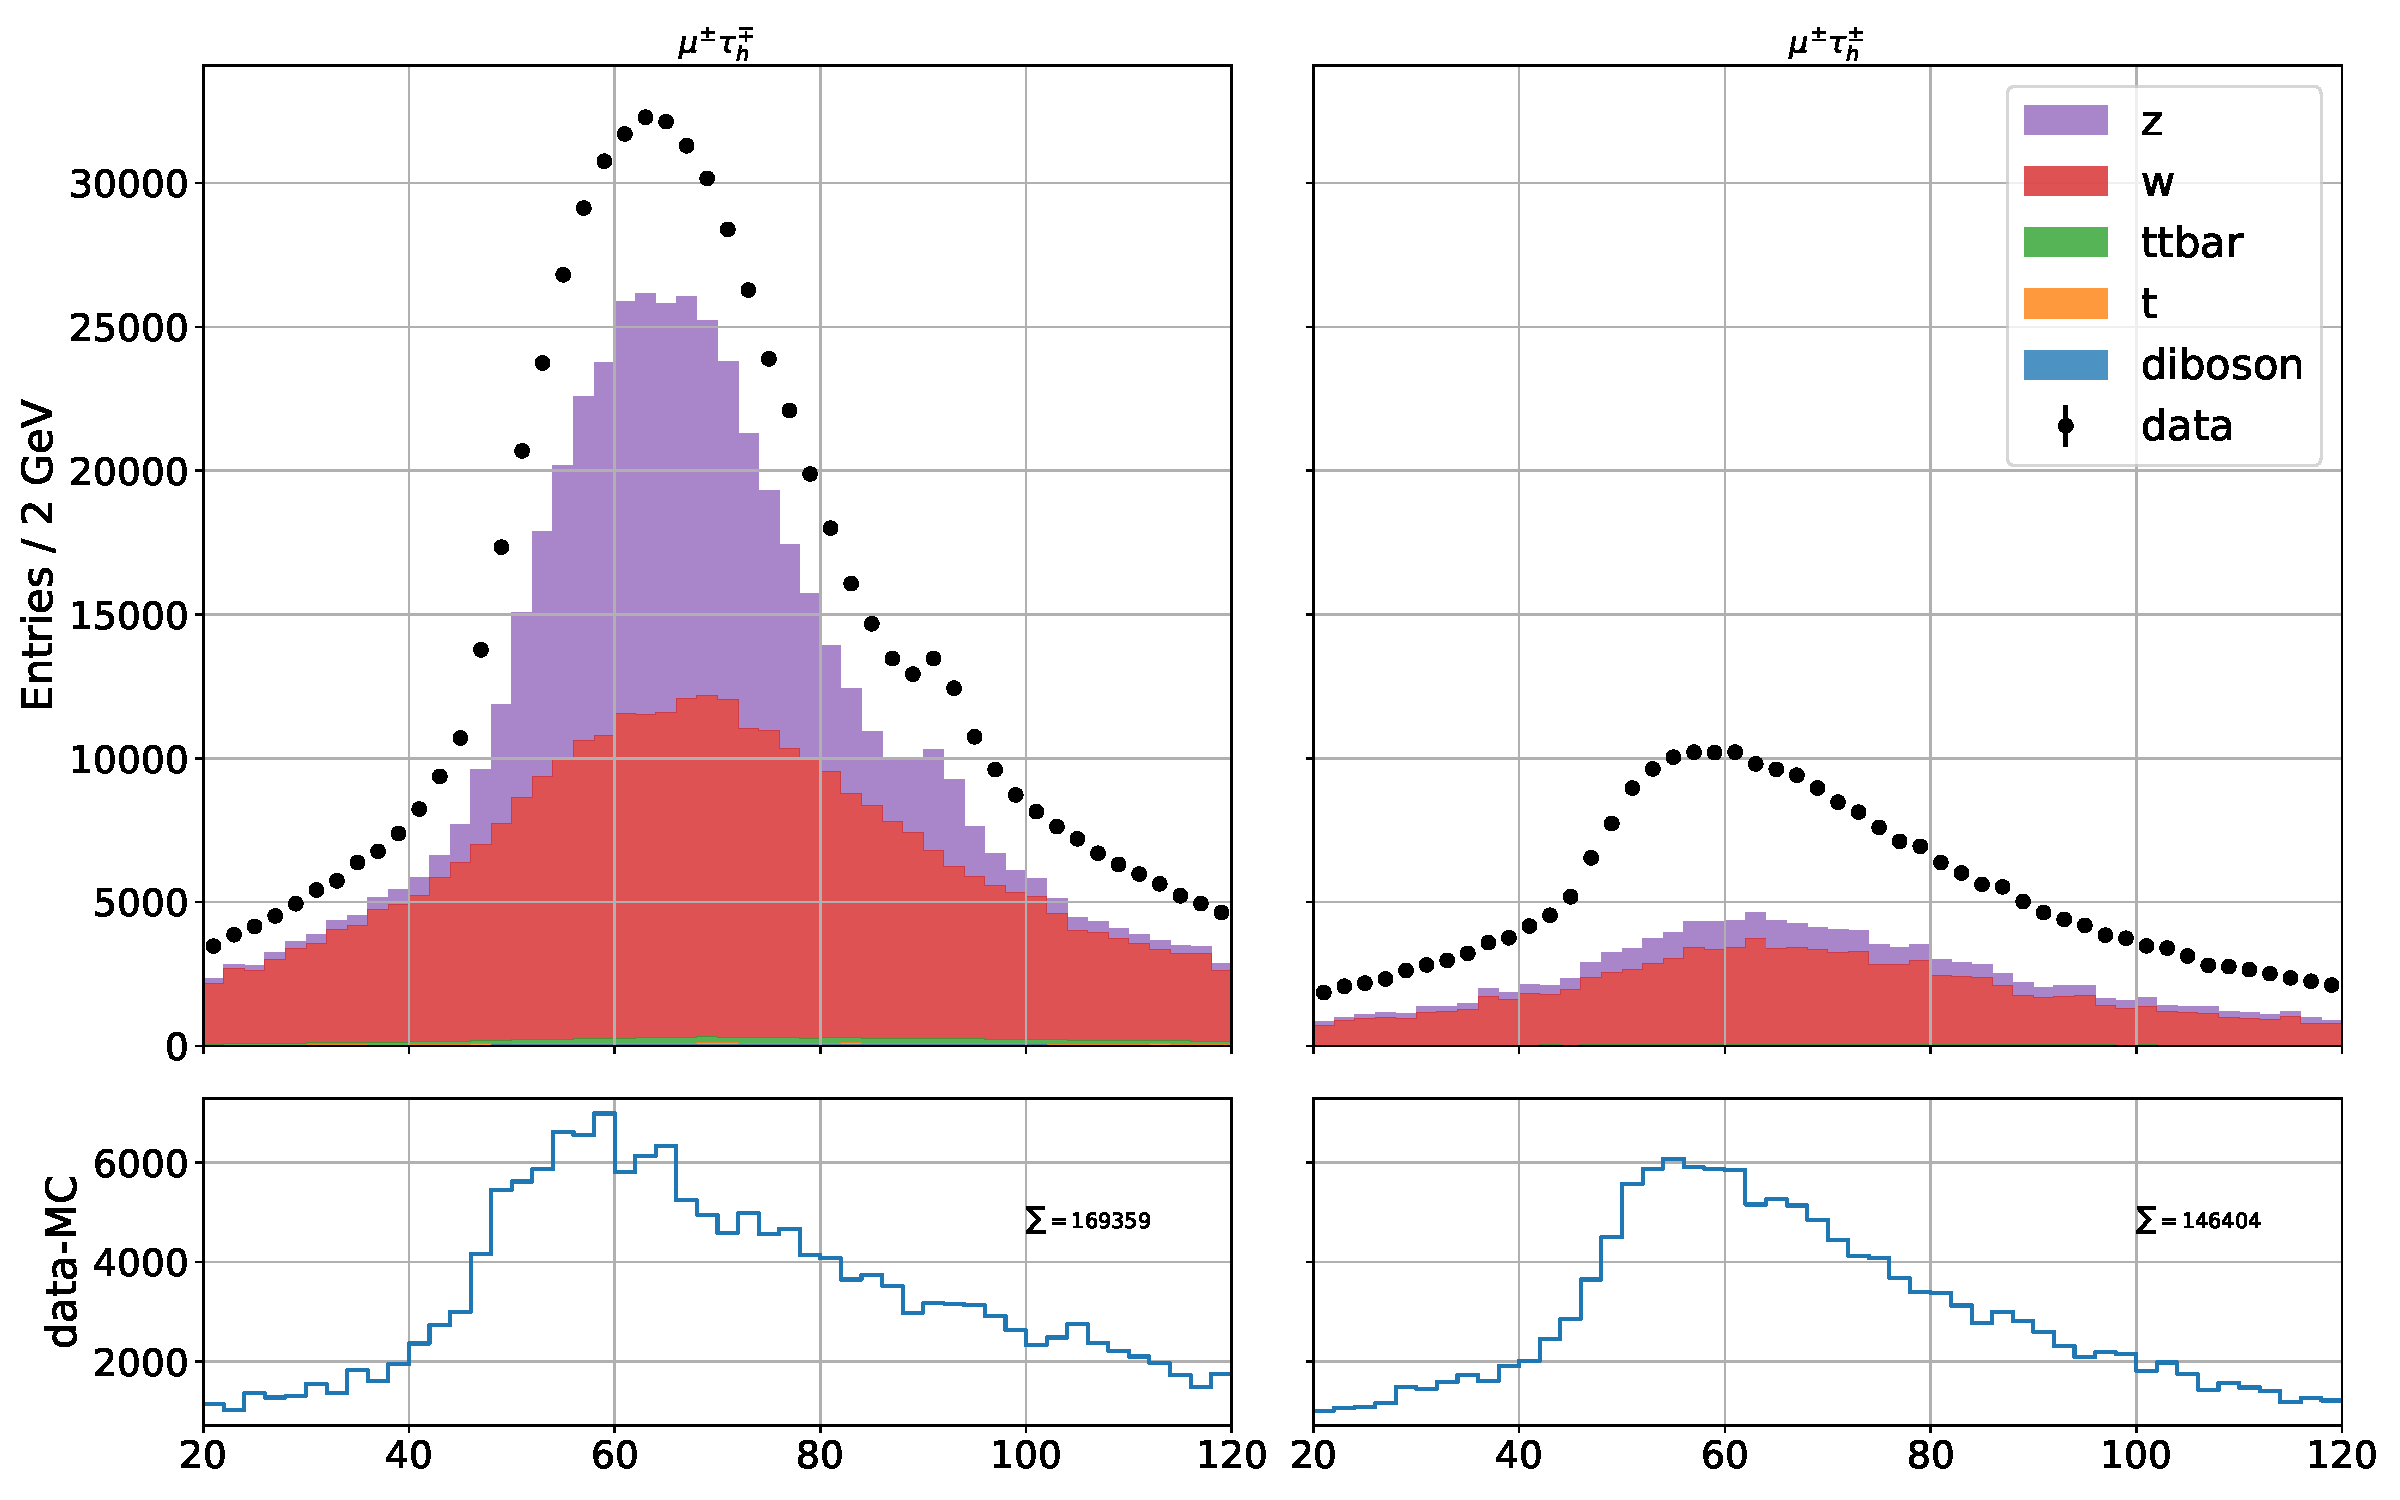
\includegraphics[width=0.49\textwidth]{chapters/Analysis/sectionBackground/figures/ltau_kinematics/mutau_cr.pdf}
    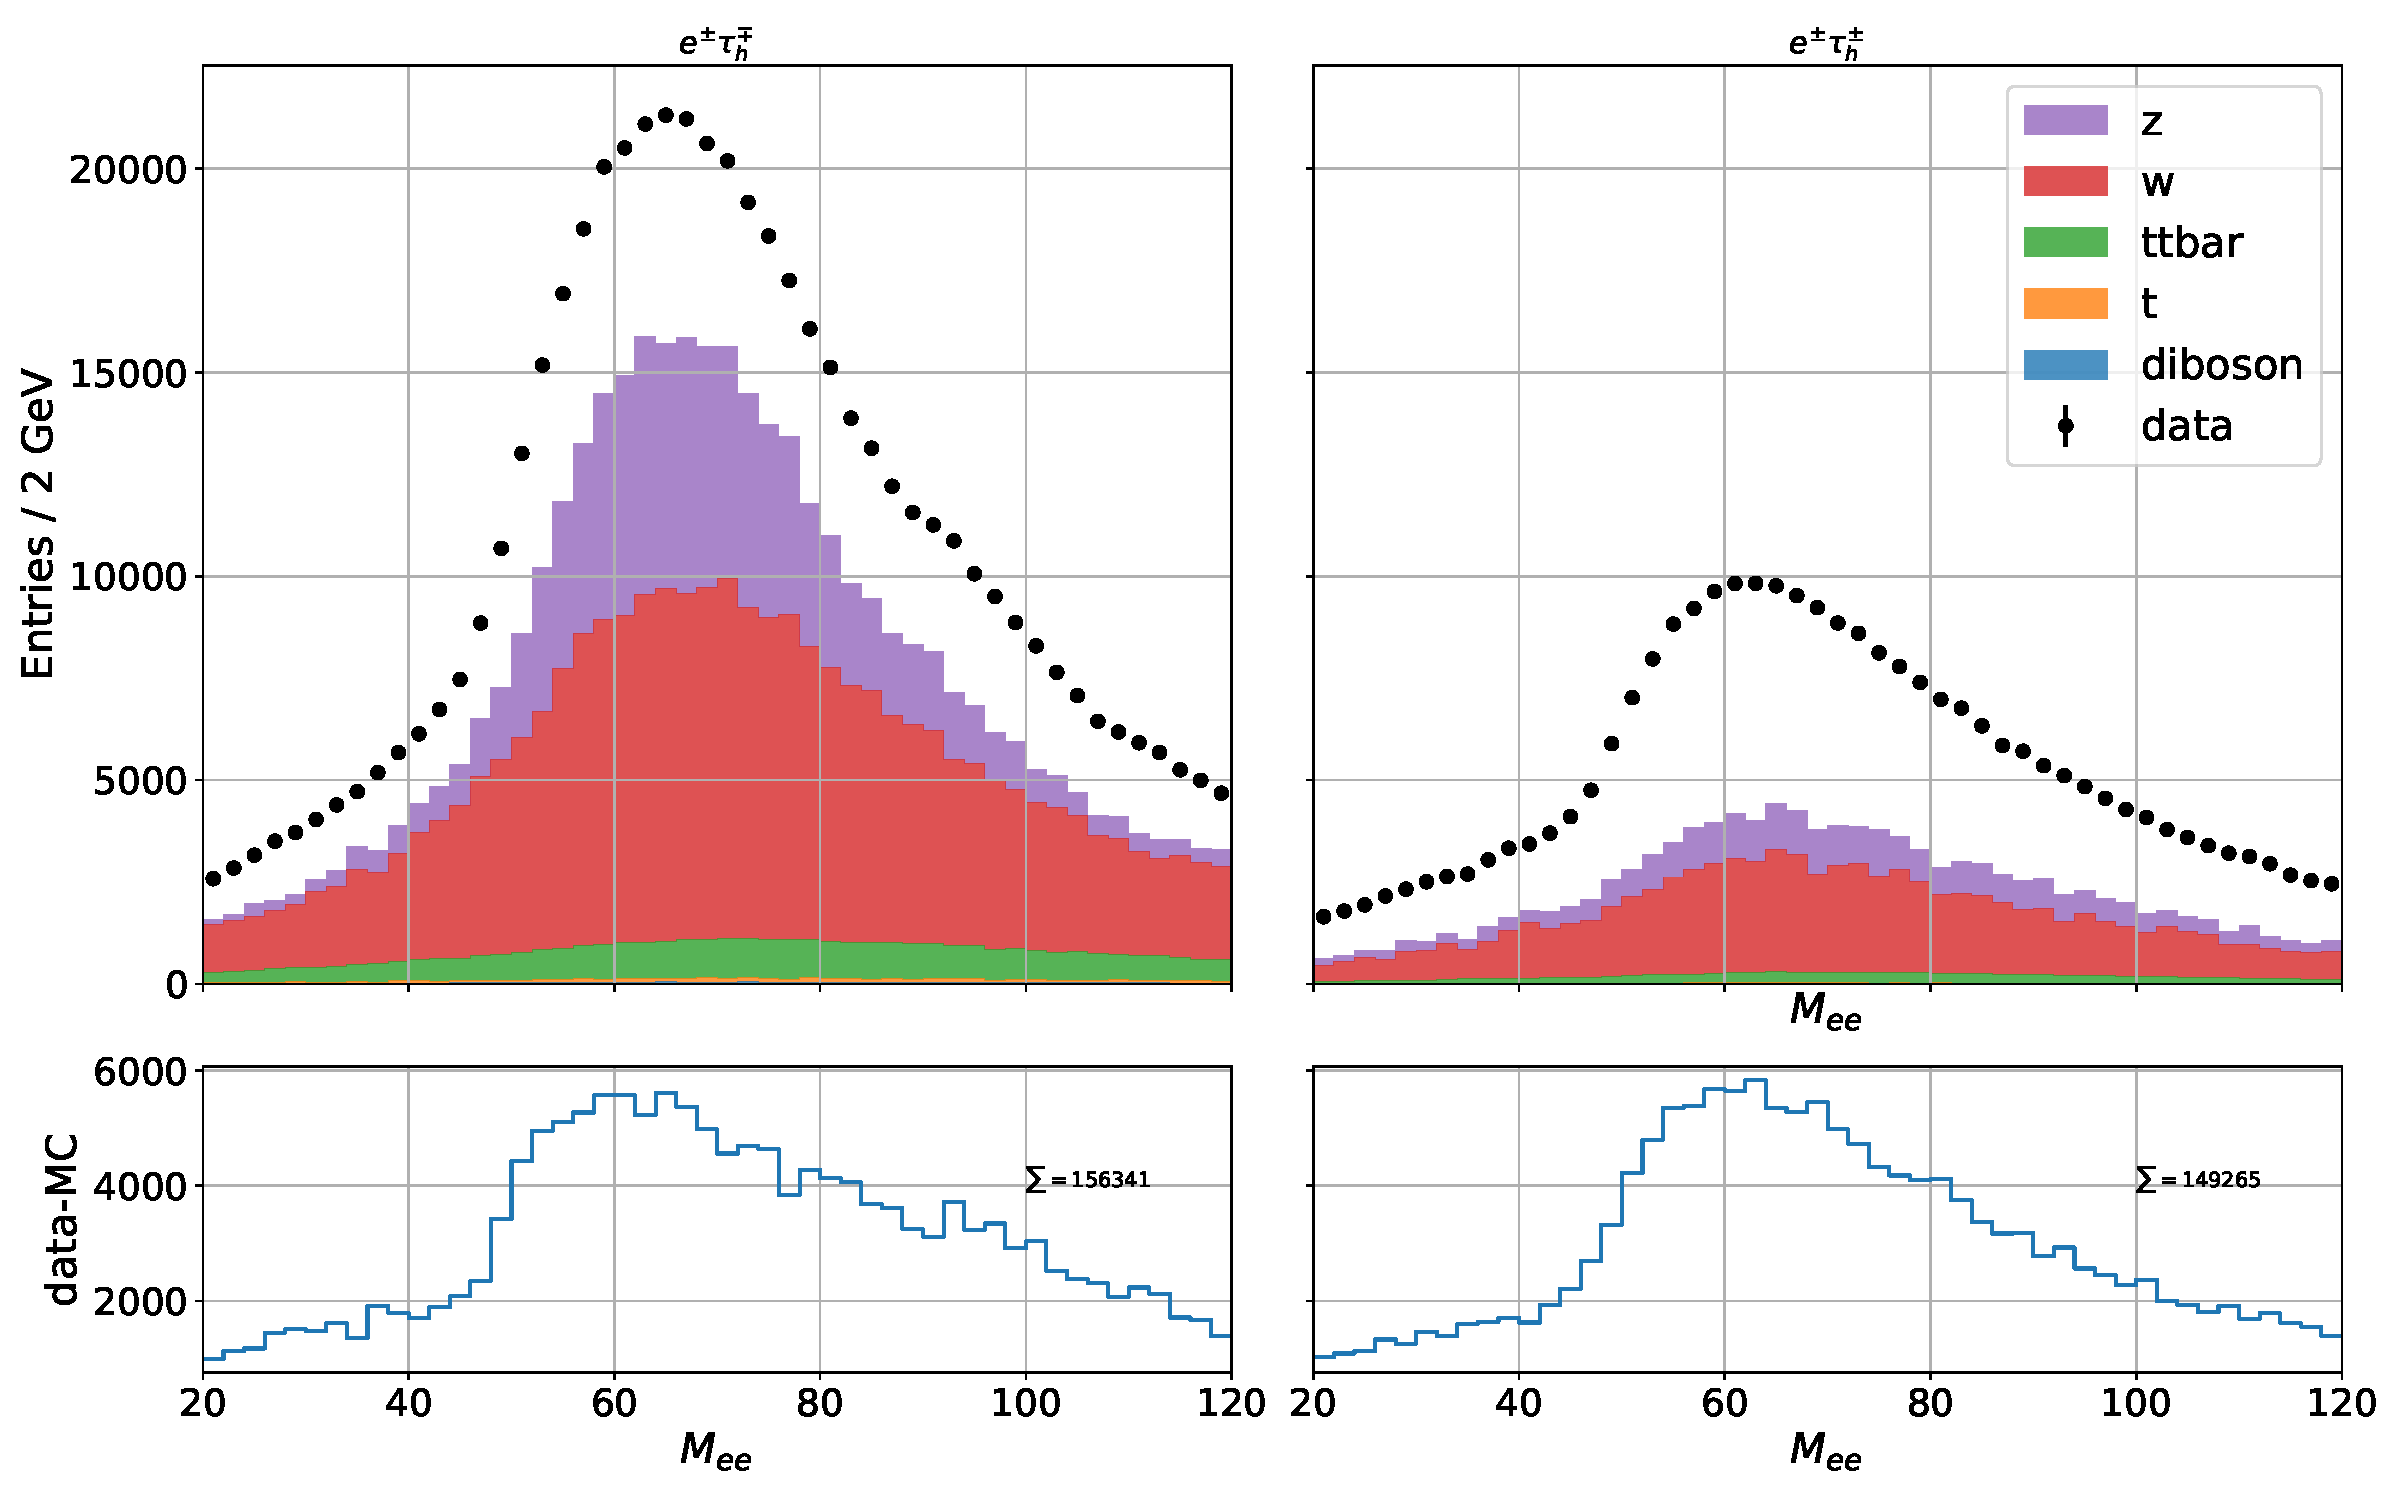
\includegraphics[width=0.49\textwidth]{chapters/Analysis/sectionBackground/figures/ltau_kinematics/etau_cr.pdf}
    \caption{The $m_{\cet}$ and $m_{\cmt}$ distributions in the same-sign and opposite-sign regions of \cet (on the right) and \cmt (on the left) channel with the anti-isolated lepton and zero jets.}
    \label{fig:background:ltau:mass_ltau_antiiso}
\end{figure}

\begin{sidewaysfigure}[h]
    \centering
    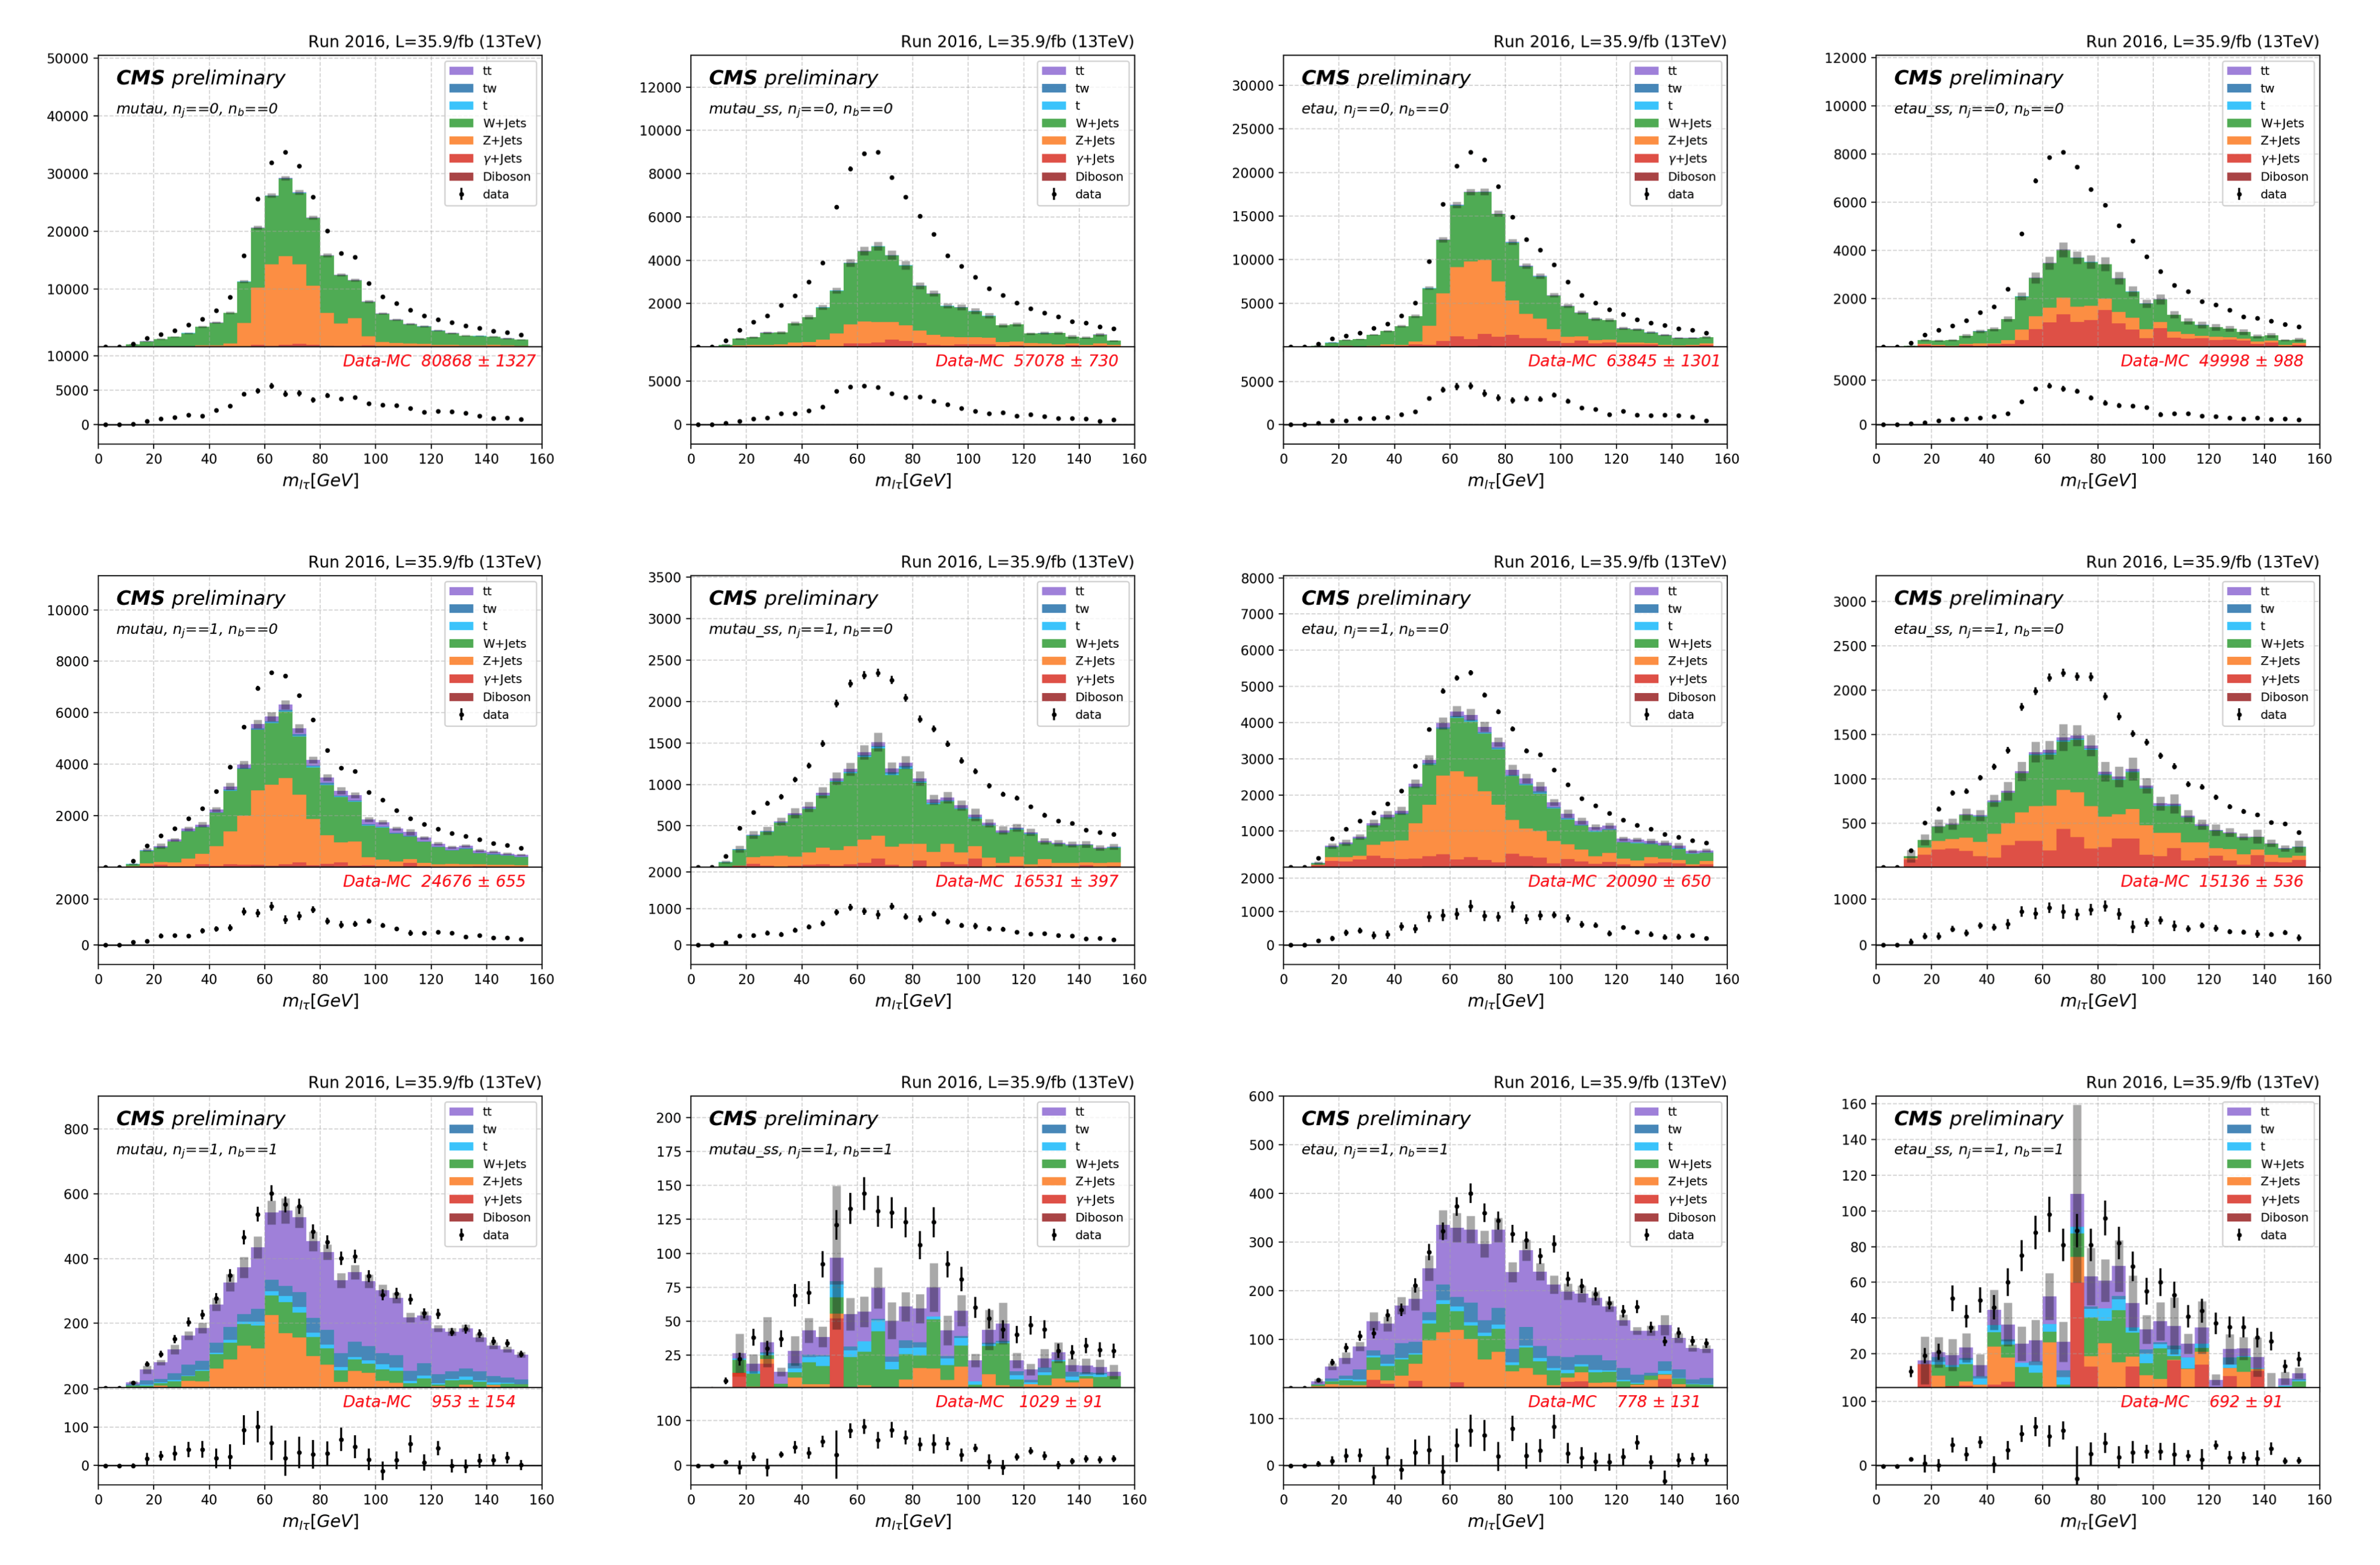
\includegraphics[width=0.9\textwidth]{chapters/Analysis/sectionBackground/figures/ltau_kinematics/ltau1.png}
    \caption{The $m_{\cmt}$ distributions in the same-sign and opposite-sign regions of \cmt channel \emph{(left two columns)}. The $m_{\cet}$ spectrum in the same-sign and opposite-sign regions of \cet channel \emph{(right two columns)}. Three rows correspond to $n_j=0,n_\PQb=0$, $n_j=1,n_\PQb=0$, $n_j=1,n_\PQb=1$, respectively. }
    \label{fig:background:ltau:mass_ltau_1}
\end{sidewaysfigure}
\begin{sidewaysfigure}[h]
    \centering
    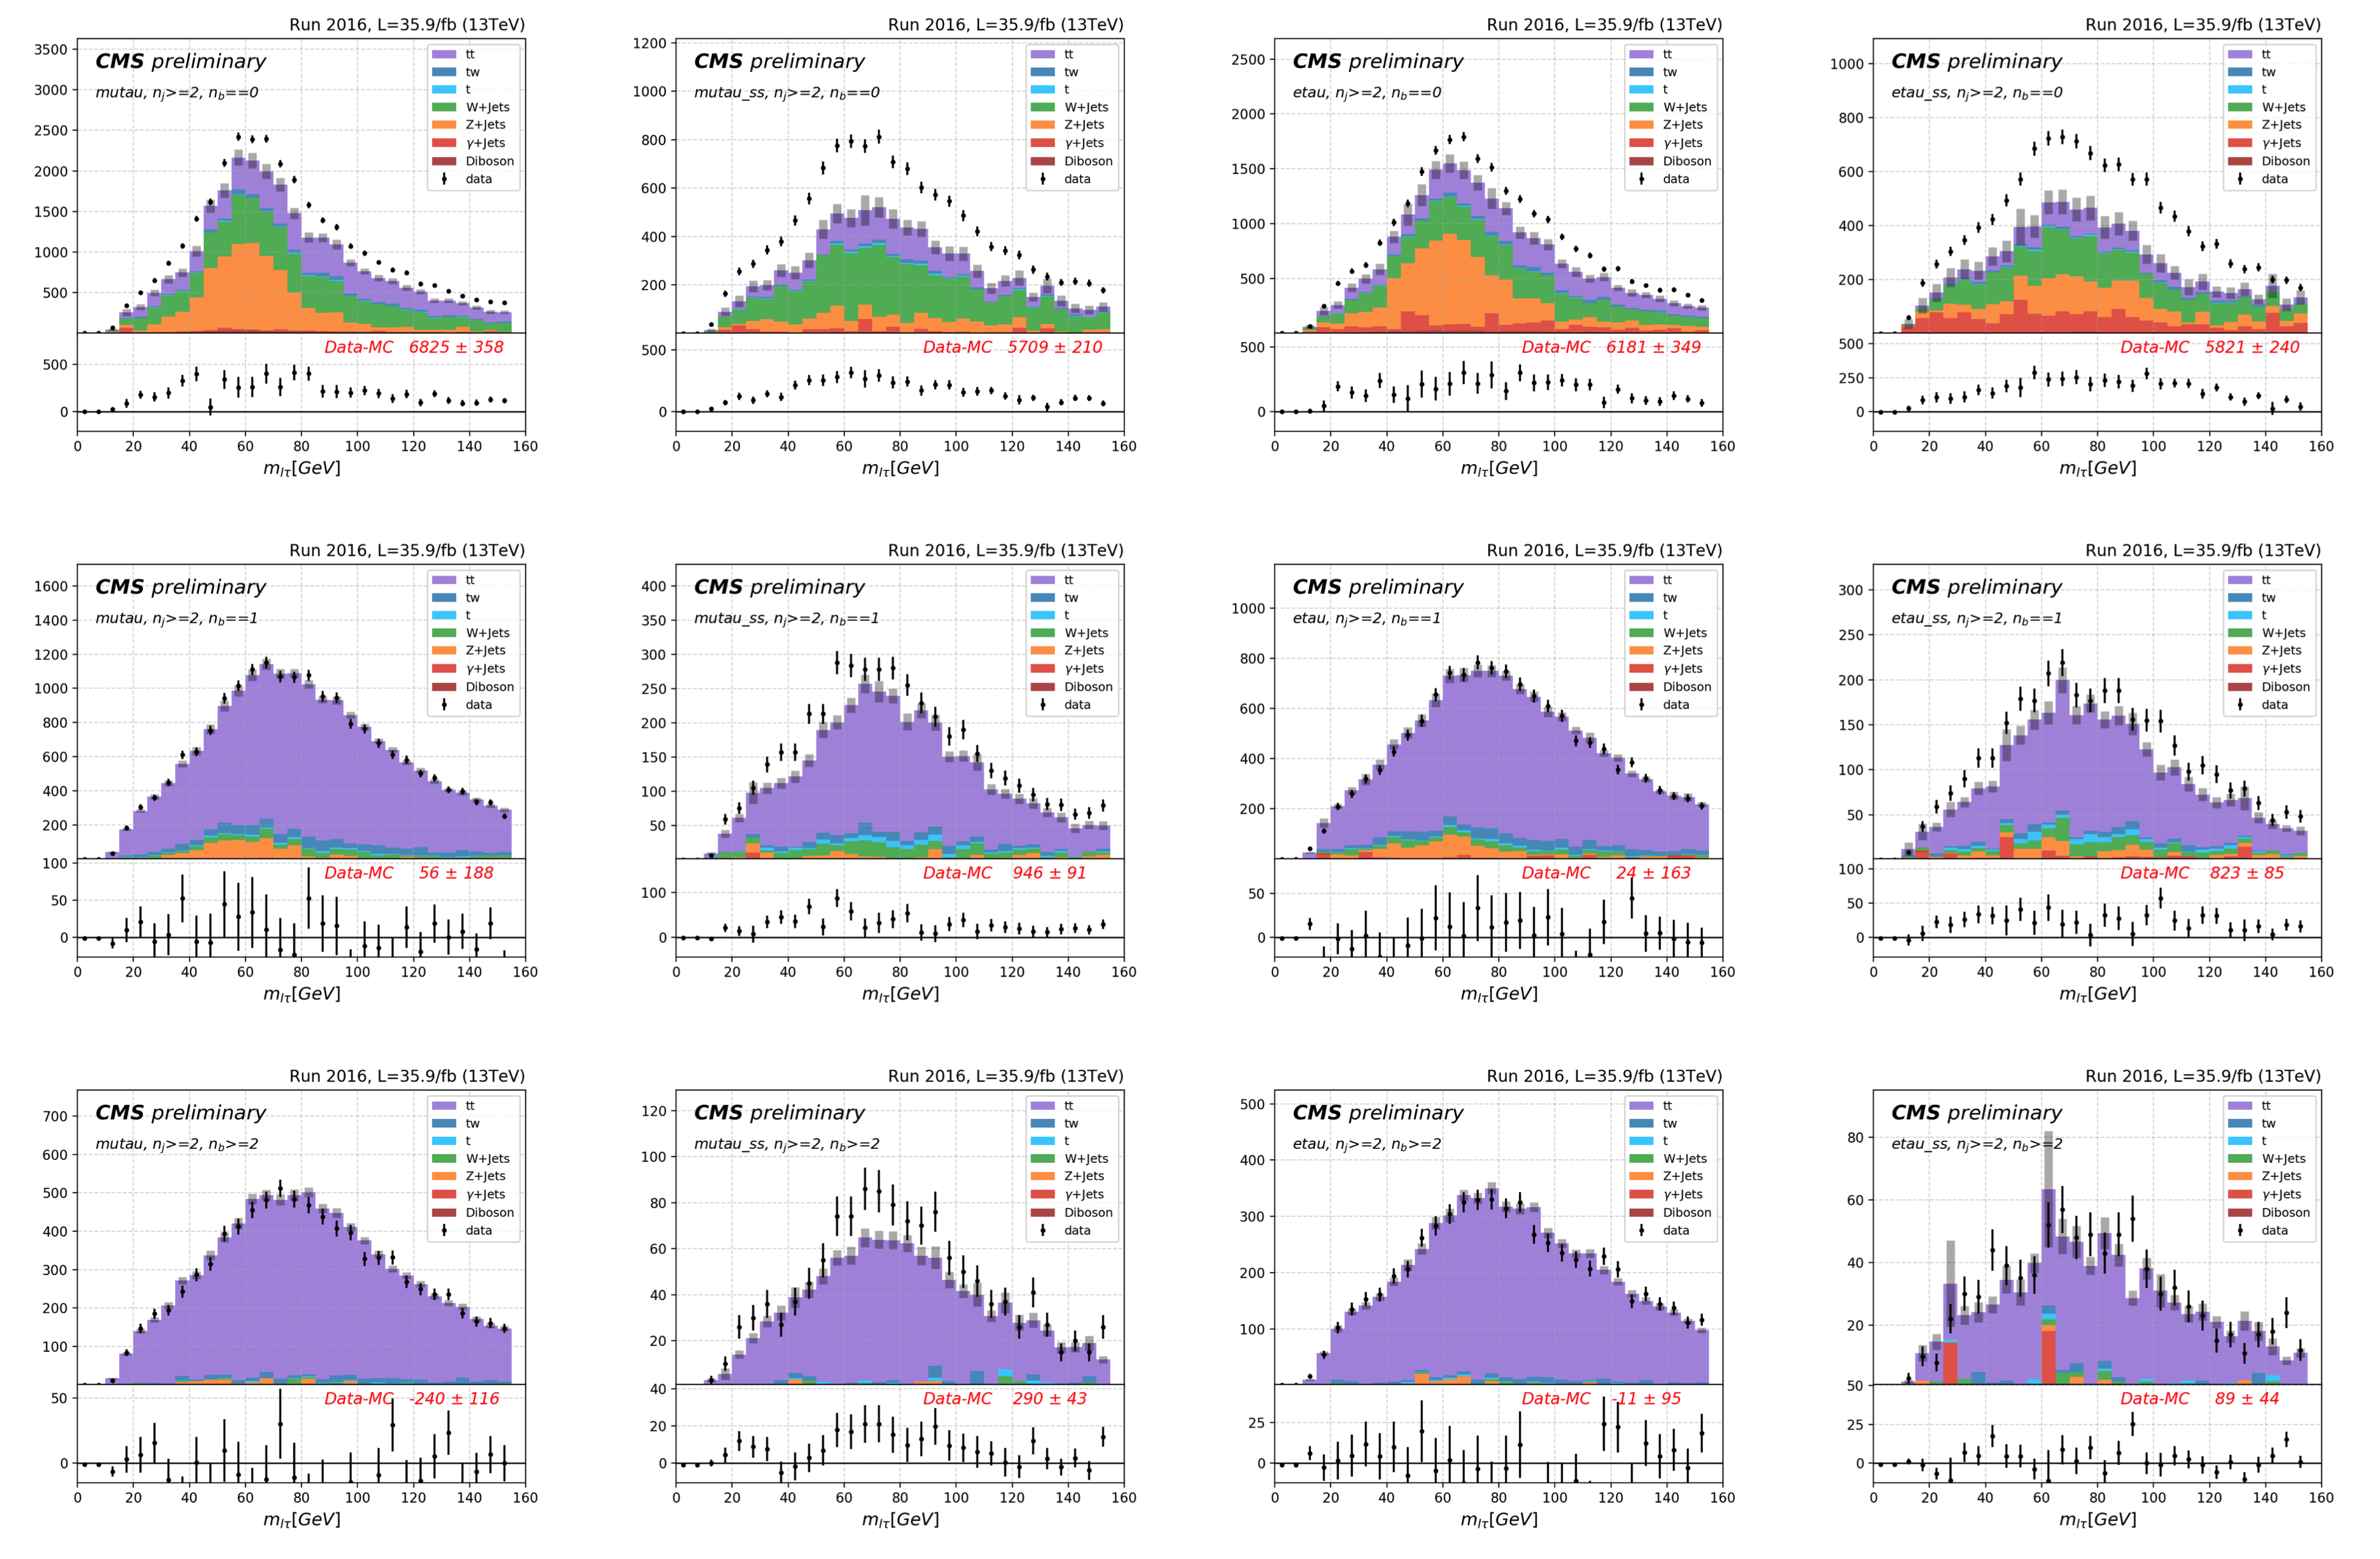
\includegraphics[width=0.9\textwidth]{chapters/Analysis/sectionBackground/figures/ltau_kinematics/ltau2.png}
    \caption{The $m_{\cmt}$ distributions in the same-sign and opposite-sign  regions of \cmt channel \emph{(left two columns)}. The $m_{\cet}$ spectrum in the same-sign and opposite-sign regions of \cet channel \emph{(right two columns)}. Three rows correspond to $n_j\geq 2,n_\PQb=0$, $n_j\geq 2,n_\PQb=1$, $n_j\geq 2,n_\PQb\geq 2$, respectively.}
    \label{fig:background:ltau:mass_ltau_2}
\end{sidewaysfigure}




\FloatBarrier





\subsection{QCD background in the $e\mathrm{h}$ and $\mu \mathrm{h}$ channels}

% A commonly used method for estimating backgrounds from misidentified prompt lepton production can be summarized as follows:

% \begin{enumerate}
%     \item construct a control region that is enhanced in the production of leptons from non-prompt sources,
    
%     \item measure the ratio, the ``fake rate", of the number of leptons passing a loose selection criteria to the number passing a tighter selection, i.e., the number of muons passing the analysis isolation requirement to those that pass with no isolation requirement,
    
%         \begin{equation}
%             f = \frac{N_{\rm pass\ iso}}{N_{\rm no iso}}
%         \end{equation}

%     \item apply a weight based on the fake rate ($w = f/(1-f)$) to events in the signal region where the leptons are required to pass the loose requirement but fail the tight requirement.
% \end{enumerate}

% The control region that is used for the fake rate measurement is selected to be enhanced in \PZ plus jet production.  Specifically, it is required that:

% \begin{itemize}
%     \item there are at least two muons or electrons passing the full analysis requirements,
%     \item the two leptons must have opposite signs,
%     \item $|M_{\ell\ell} - M_{Z}| < 15~\GeV$,
%     \item the dilepton pair that has mass closest to the \PZ boson is selected
%     \item one additional lepton (muon or electron) passing all
%     identification requirements except the isolation requirement
% \end{itemize}

% The additional lepton is assumed to originate from an hadronic jet that is produced in association with the \PZ boson, but can frequently arise due to a prompt lepton produced from a diboson process such as WZ or ZZ production.  This is accounted for by subtracting off the estimate of these processes from simulation from the data in the fake rate control region.  Figures~\ref{fig:lepton_fr} show the measured \pt distributions of the electron and muon candidates and the resulting fake rates and the values for each of the \pt bins are shown in table~\ref{tab:lepton_fr}.



% The fake rate that is applied to the data in the isolation sideband of the signal region is the one derived from data.  The systematic uncertainty on this background is conservatively treated as being 30\% for both electron and muon fakes.  





In the \ceh and \cmh channels, the QCD estimations are based on side-band regions with inverted lepton isolation, where the data excess with respective to the simulations are multiplied by an anti-isolation ($\rm \overline{iso}$) to isolation (iso) transfer factor depending on the lepton \pt and $\eta$. When selecting anti-isolated electrons and muons, the isolation is required to pass loose working point but fail the tight working point. The requirement of single lepton trigger is the same as the isolated lepton cases. 

The anti-isolation to isolation transfer factor is defined as 
\begin{equation}
SF^{\rm \overline{iso} \to iso} (\pt, \eta) =  \frac{N^{\rm iso}_{\rm data} (\pt, \eta) - \sum N^{\rm iso}_{\rm MC}(\pt, \eta) } {N^{\rm \overline{iso}}_{\rm data} (\pt, \eta)- \sum N^{\rm \overline{iso}}_{\rm MC}(\pt, \eta) }
\end{equation}
\noindent To measure $SF^{\rm \overline{iso} \to iso}$, an orthogonal region with lepton plus $1\leq n_j<4$ and $n_\PQb\geq1$ is considered. To reduce the contamination for \wjets and enhance the QCD purity, $m_{\rm T}^{\ell, MET} < 40 \GeV$ is required. Figure~\ref{fig:background:lh:123j1b} shows the isolated and anti-isolated lepton plus jet regions with $1\leq n_j<4$ and $n_\PQb\geq1$, \cmh in the left two columns and \ceh in the right two columns. The measured $SF^{\rm \overline{iso} \to iso}$ result is shown in Figure~\ref{fig:background:lh:123j1b_sf}. 
\begin{figure}
    \centering
    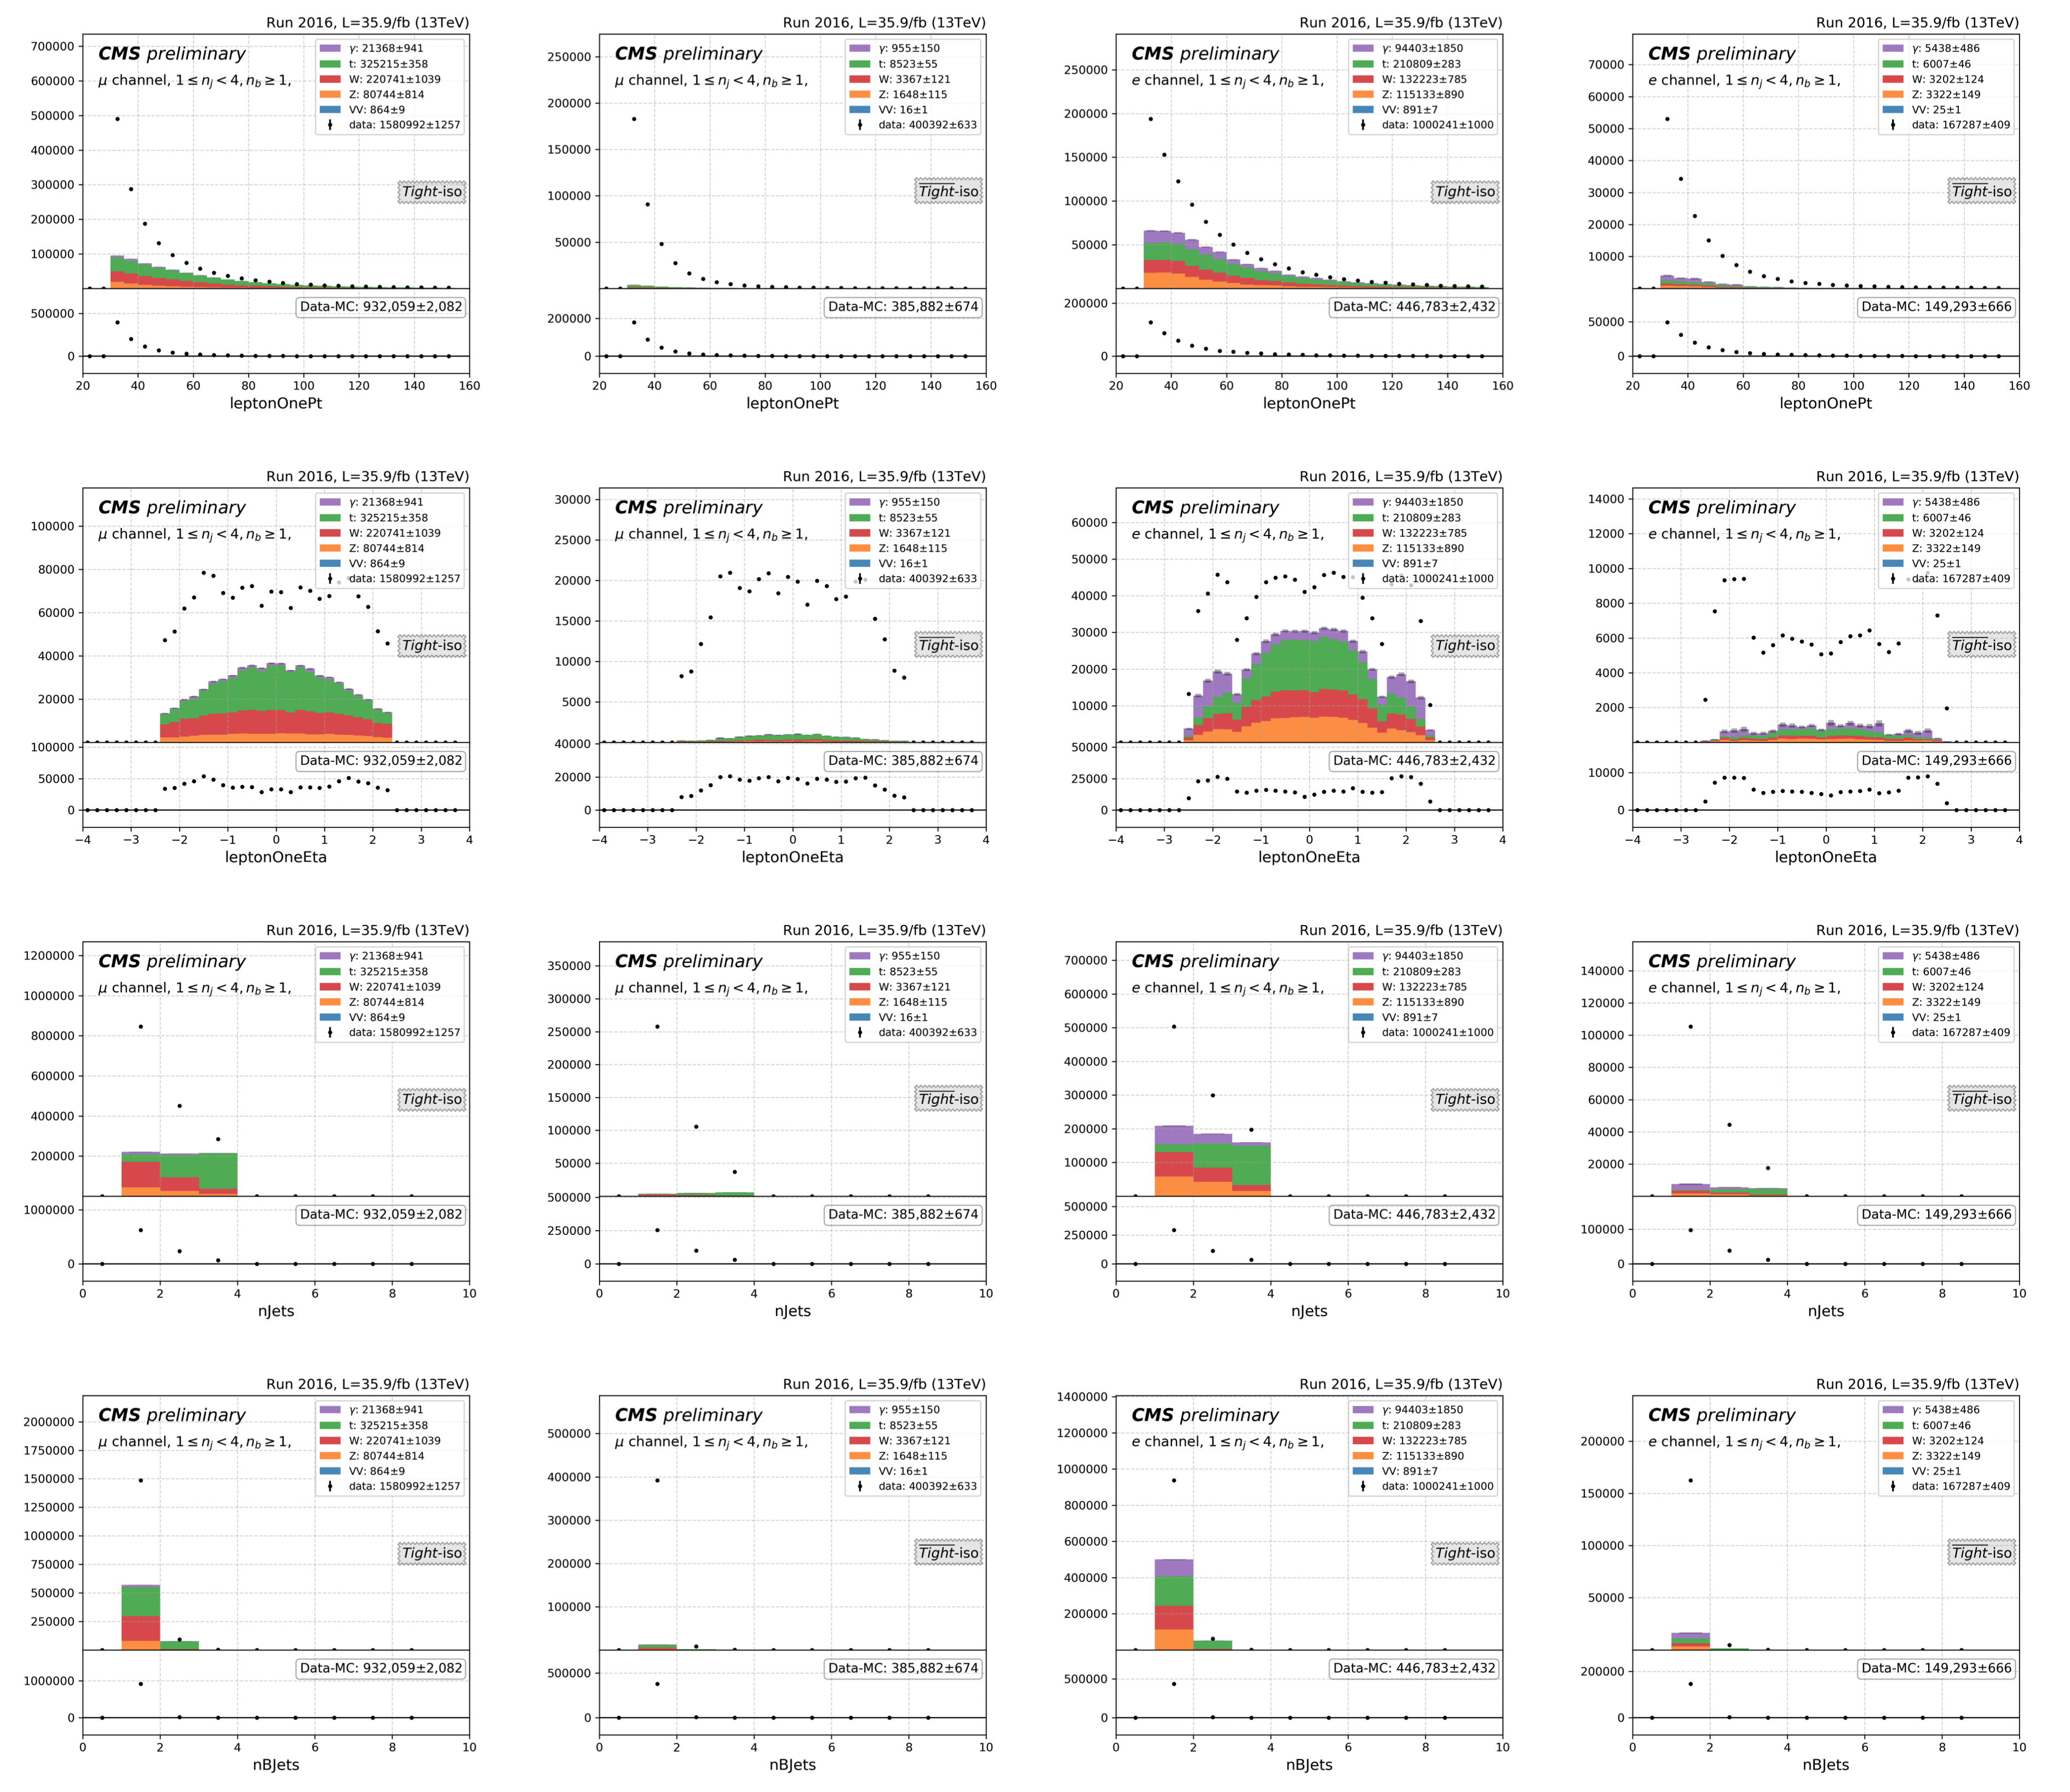
\includegraphics[width=0.99\textwidth]{chapters/Analysis/sectionBackground/figures/ljets_kinematics/123j1b.png}
    \caption{isolated and anti-isolated lepton plus jet regions with $1\leq n_j<4$ and $n_\PQb\geq1$, \cmh in the left two columns and \ceh in the right two columns.}
    \label{fig:background:lh:123j1b}
\end{figure}
\begin{figure}
    \centering
    % 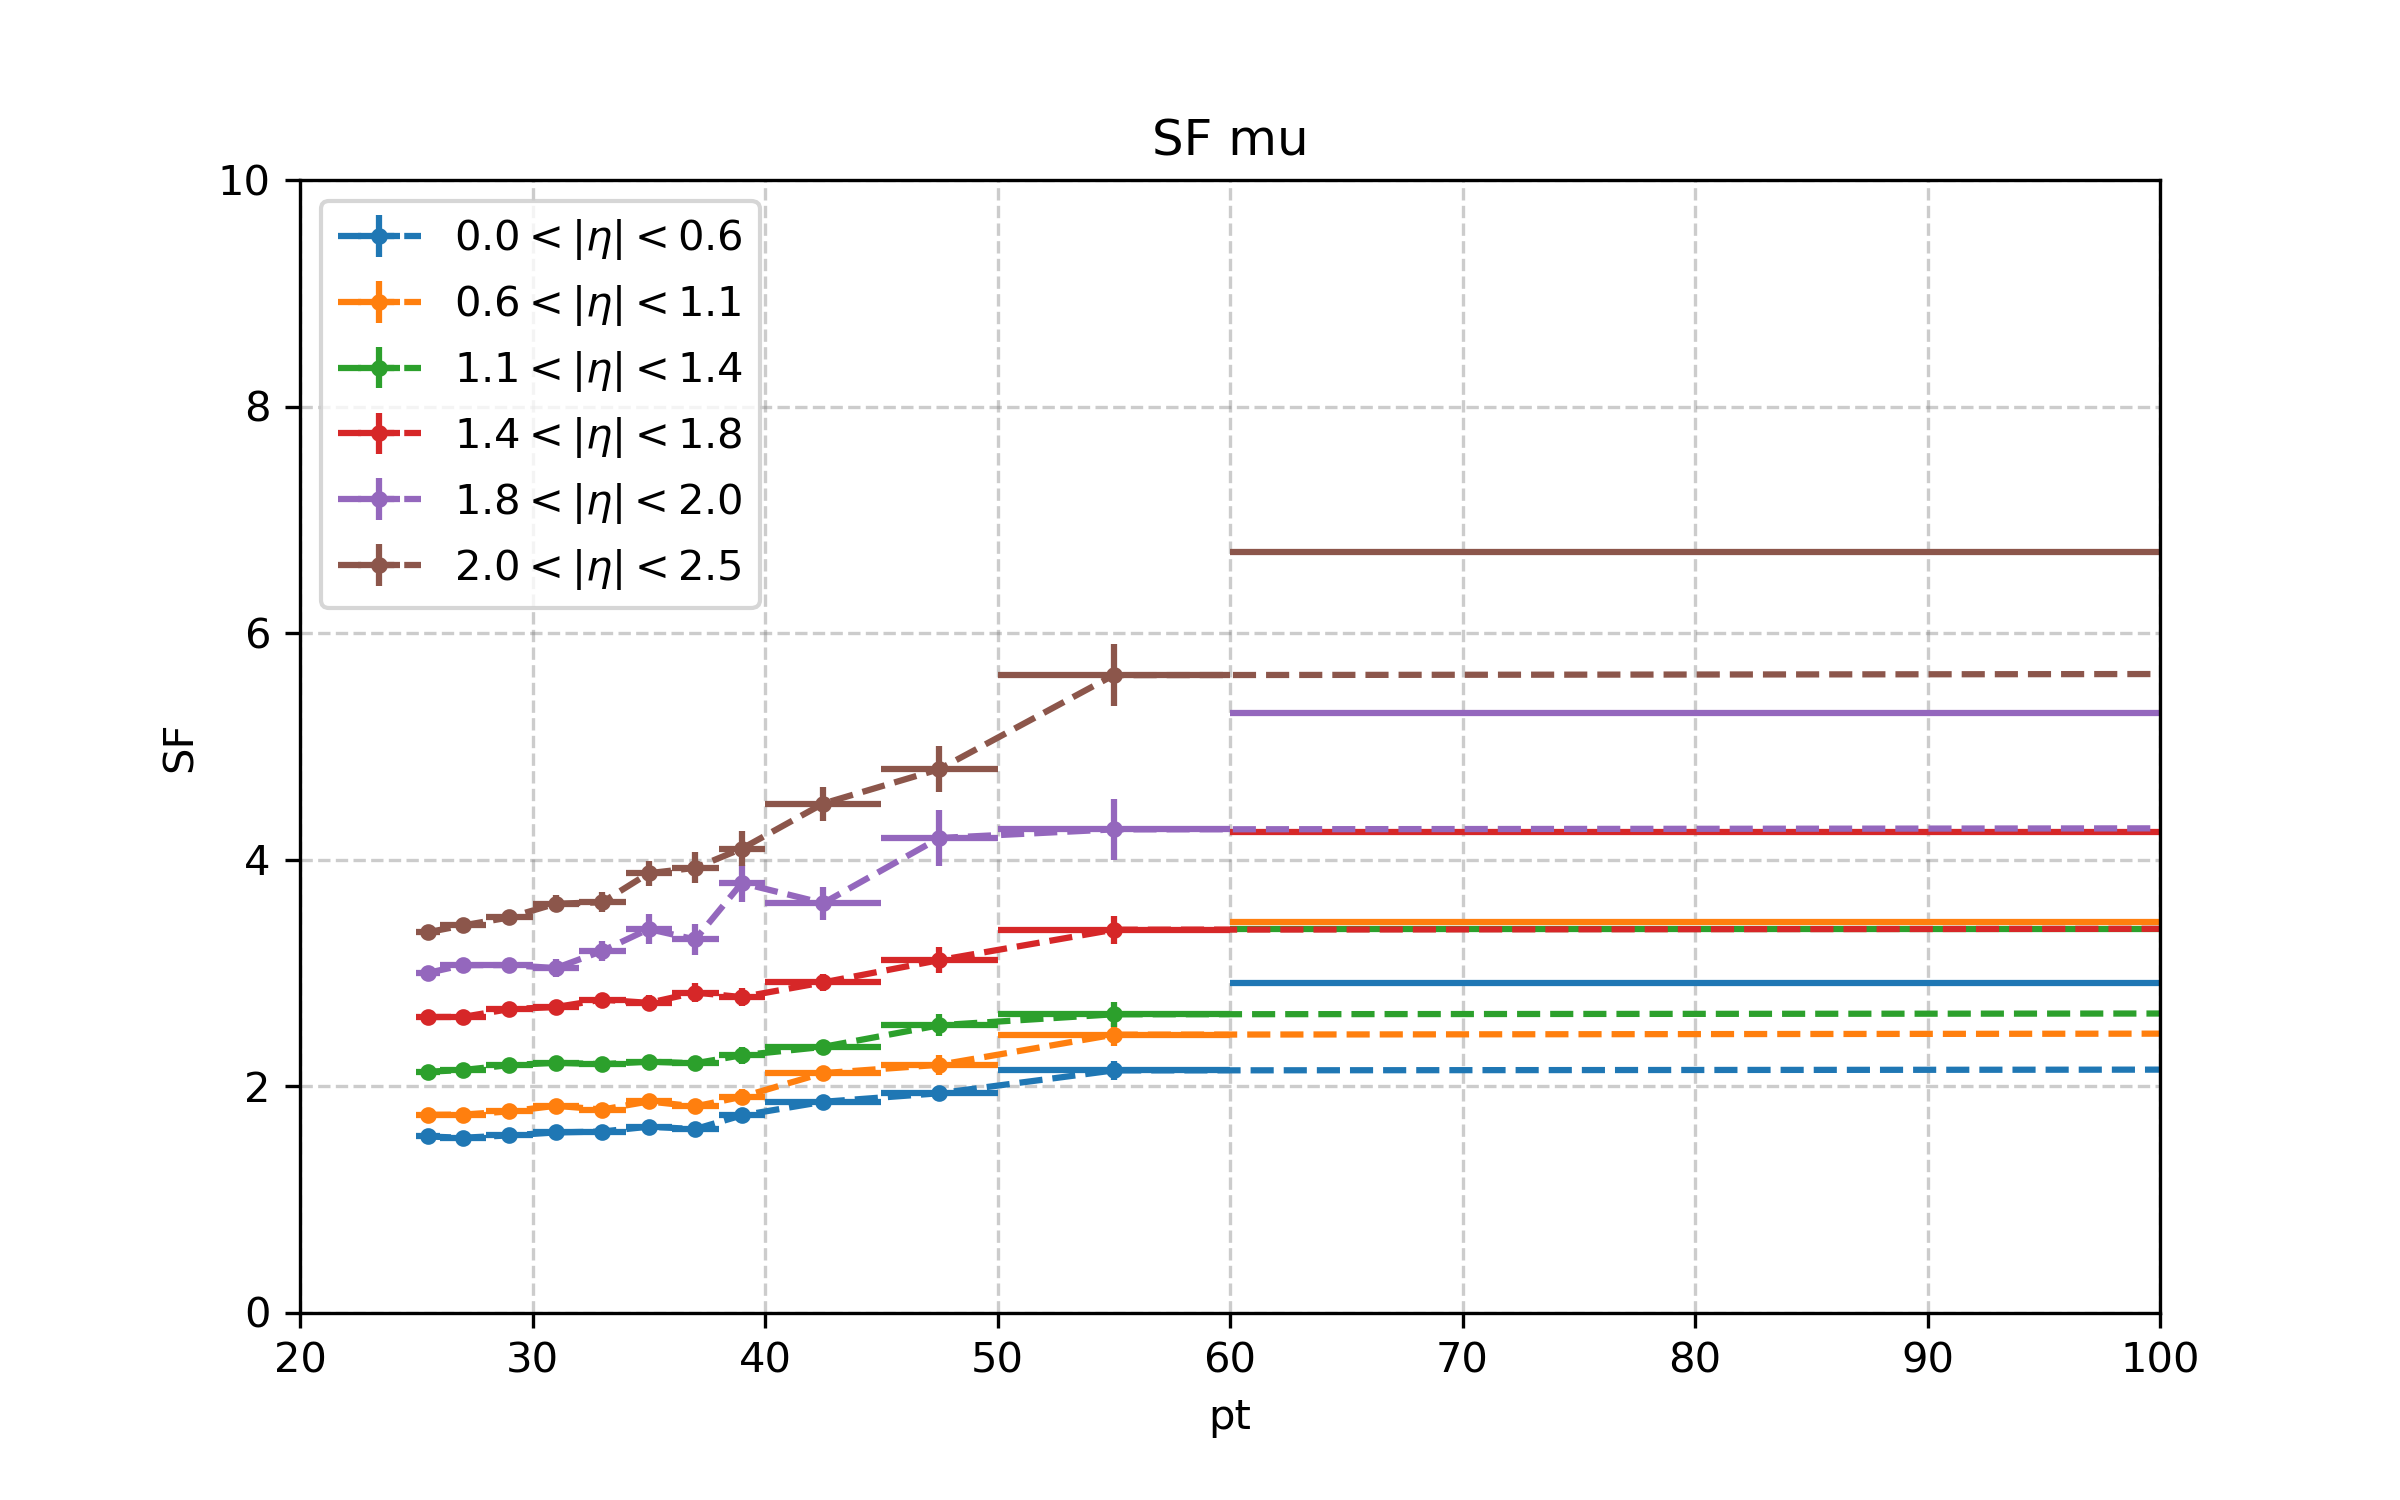
\includegraphics[width=0.49\textwidth]{chapters/Analysis/sectionBackground/figures/ljets_kinematics/123j1b/SF_mu_1d.png}
    % 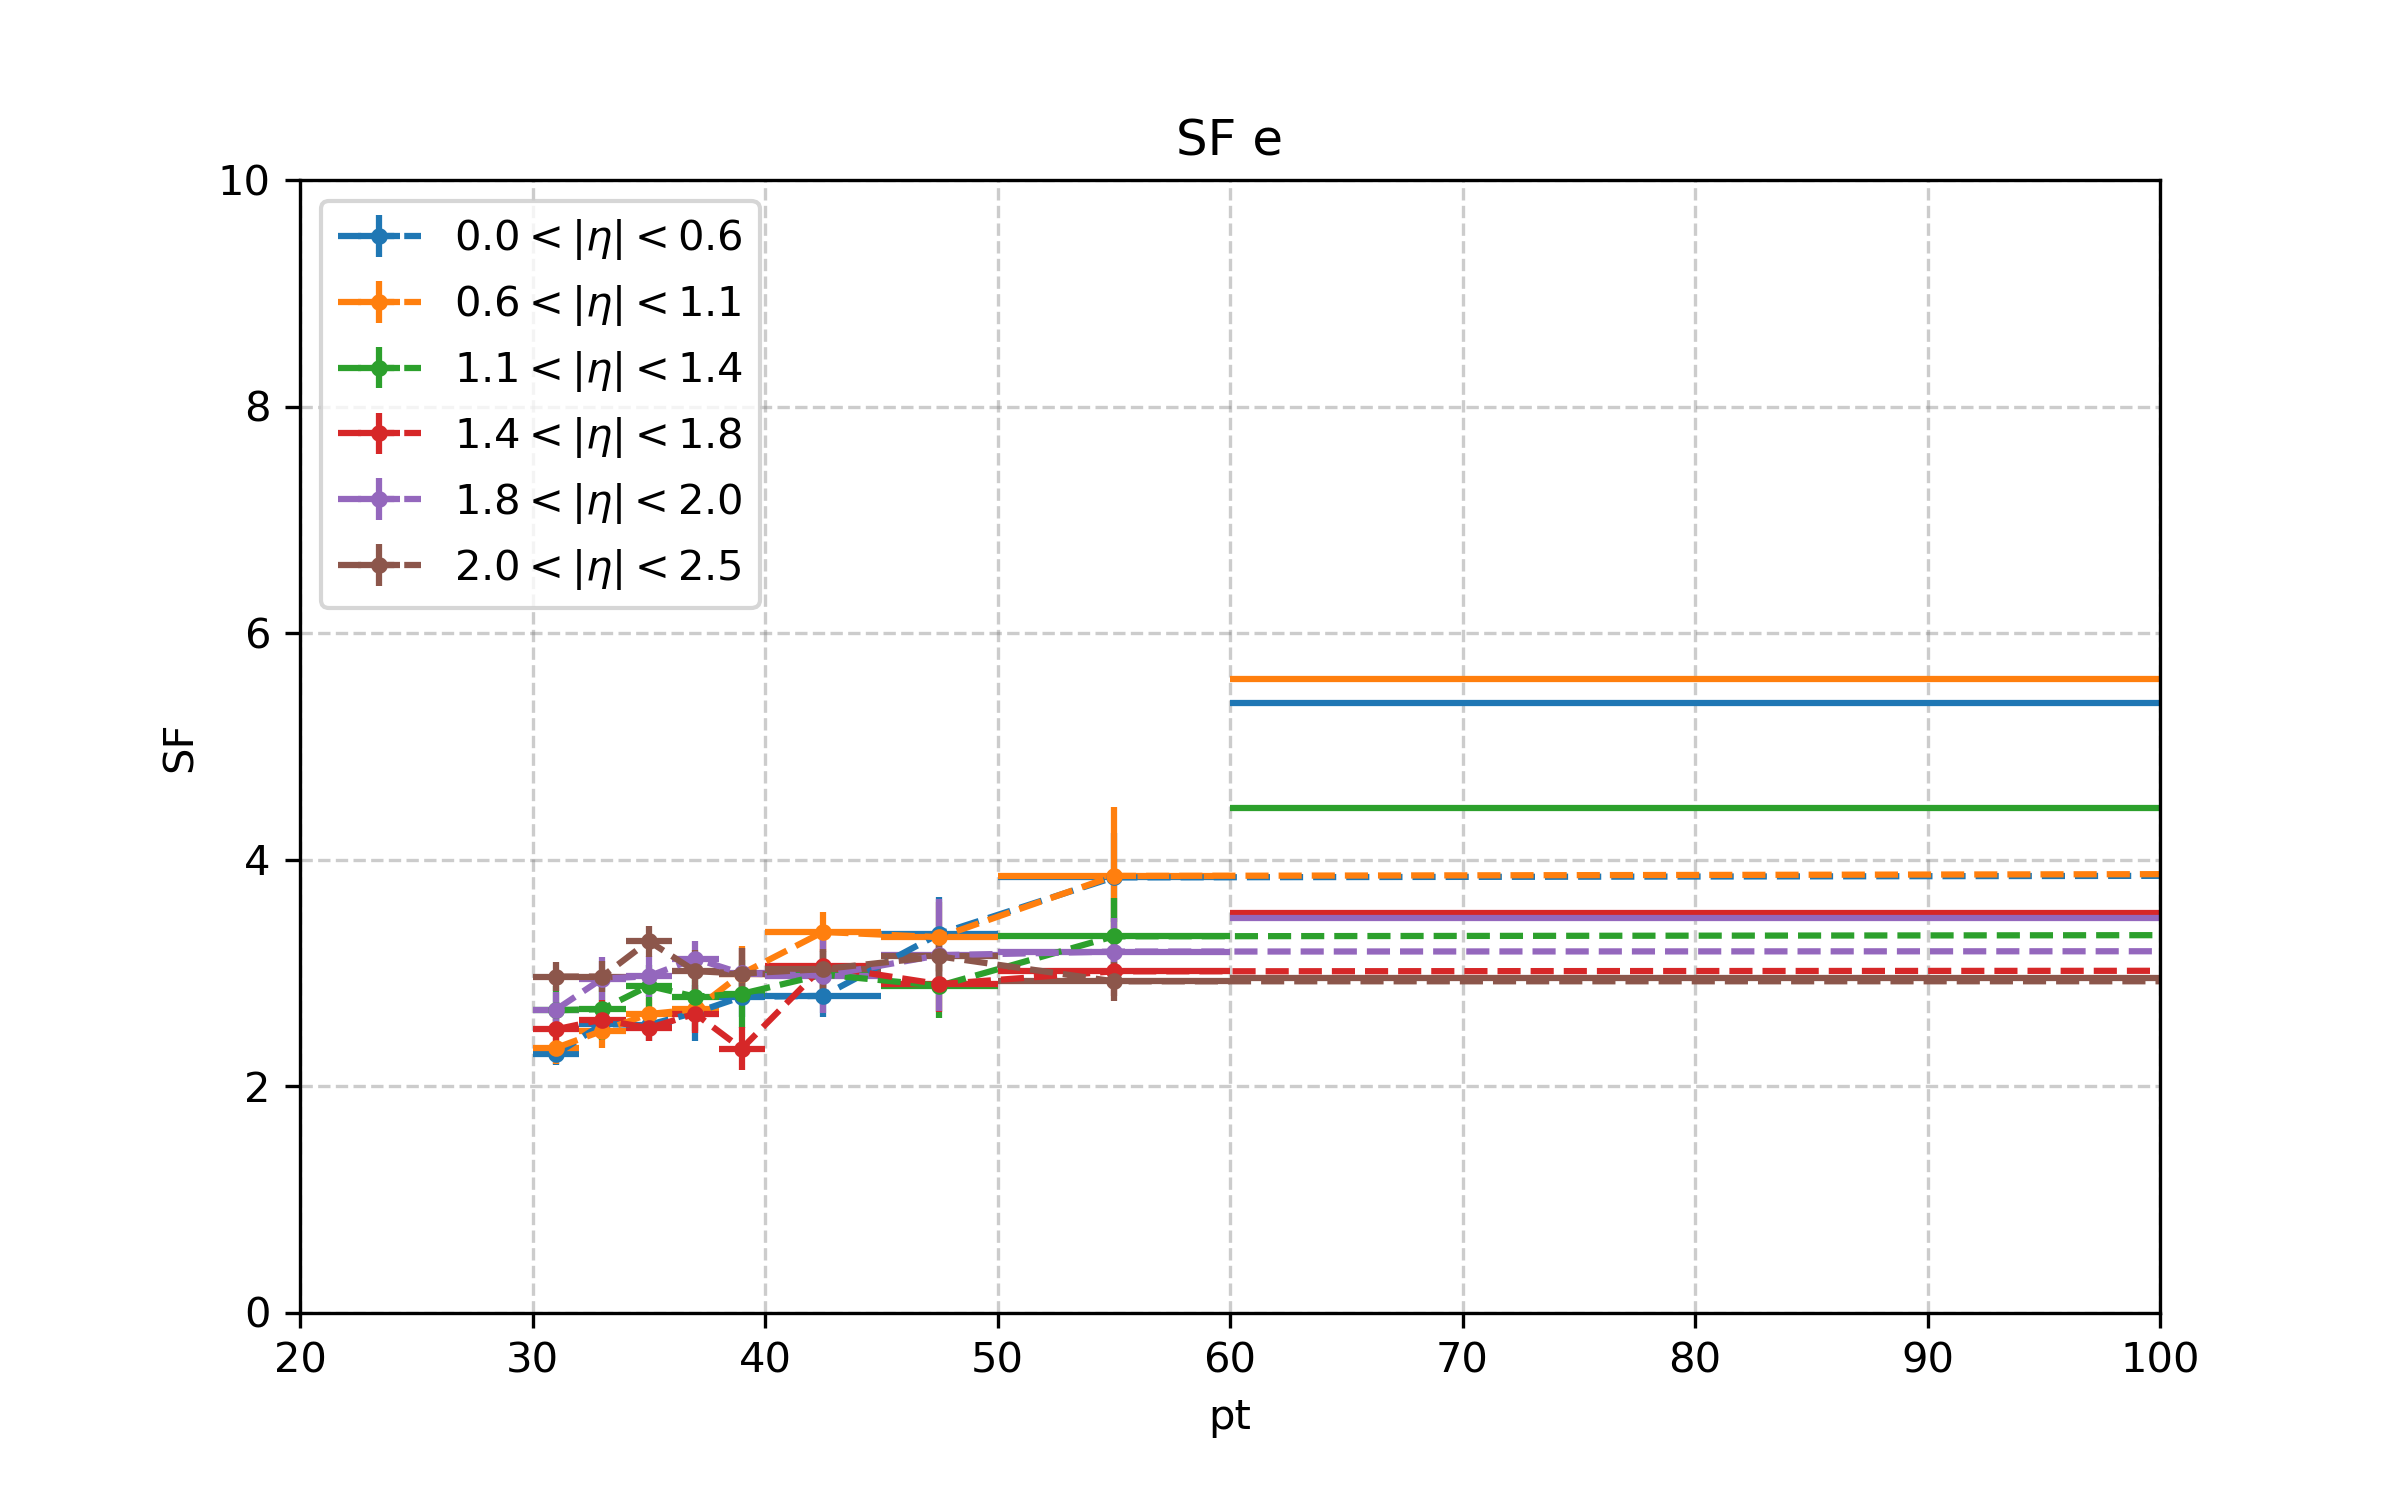
\includegraphics[width=0.49\textwidth]{chapters/Analysis/sectionBackground/figures/ljets_kinematics/123j1b/SF_e_1d.png}
    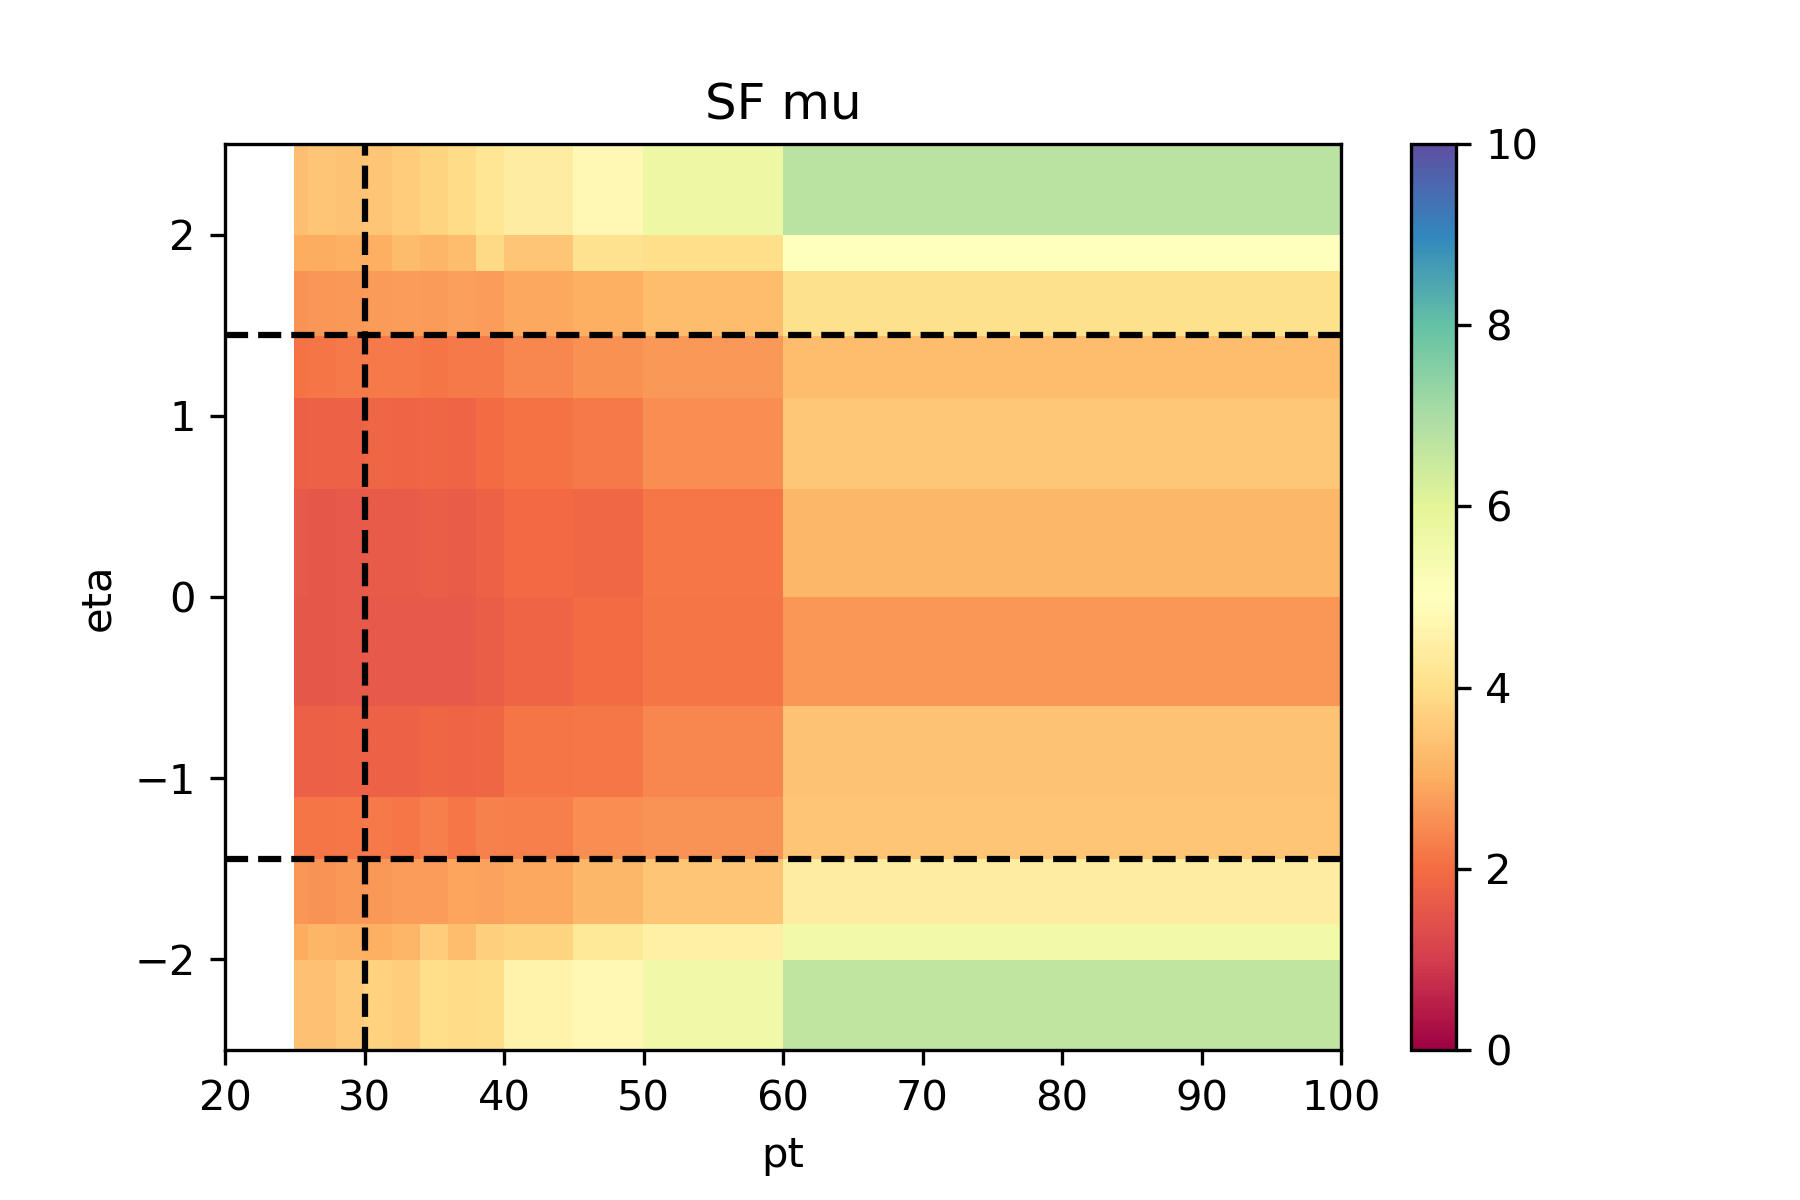
\includegraphics[width=0.49\textwidth]{chapters/Analysis/sectionBackground/figures/ljets_kinematics/123j1b/SF_mu_2d.png}
    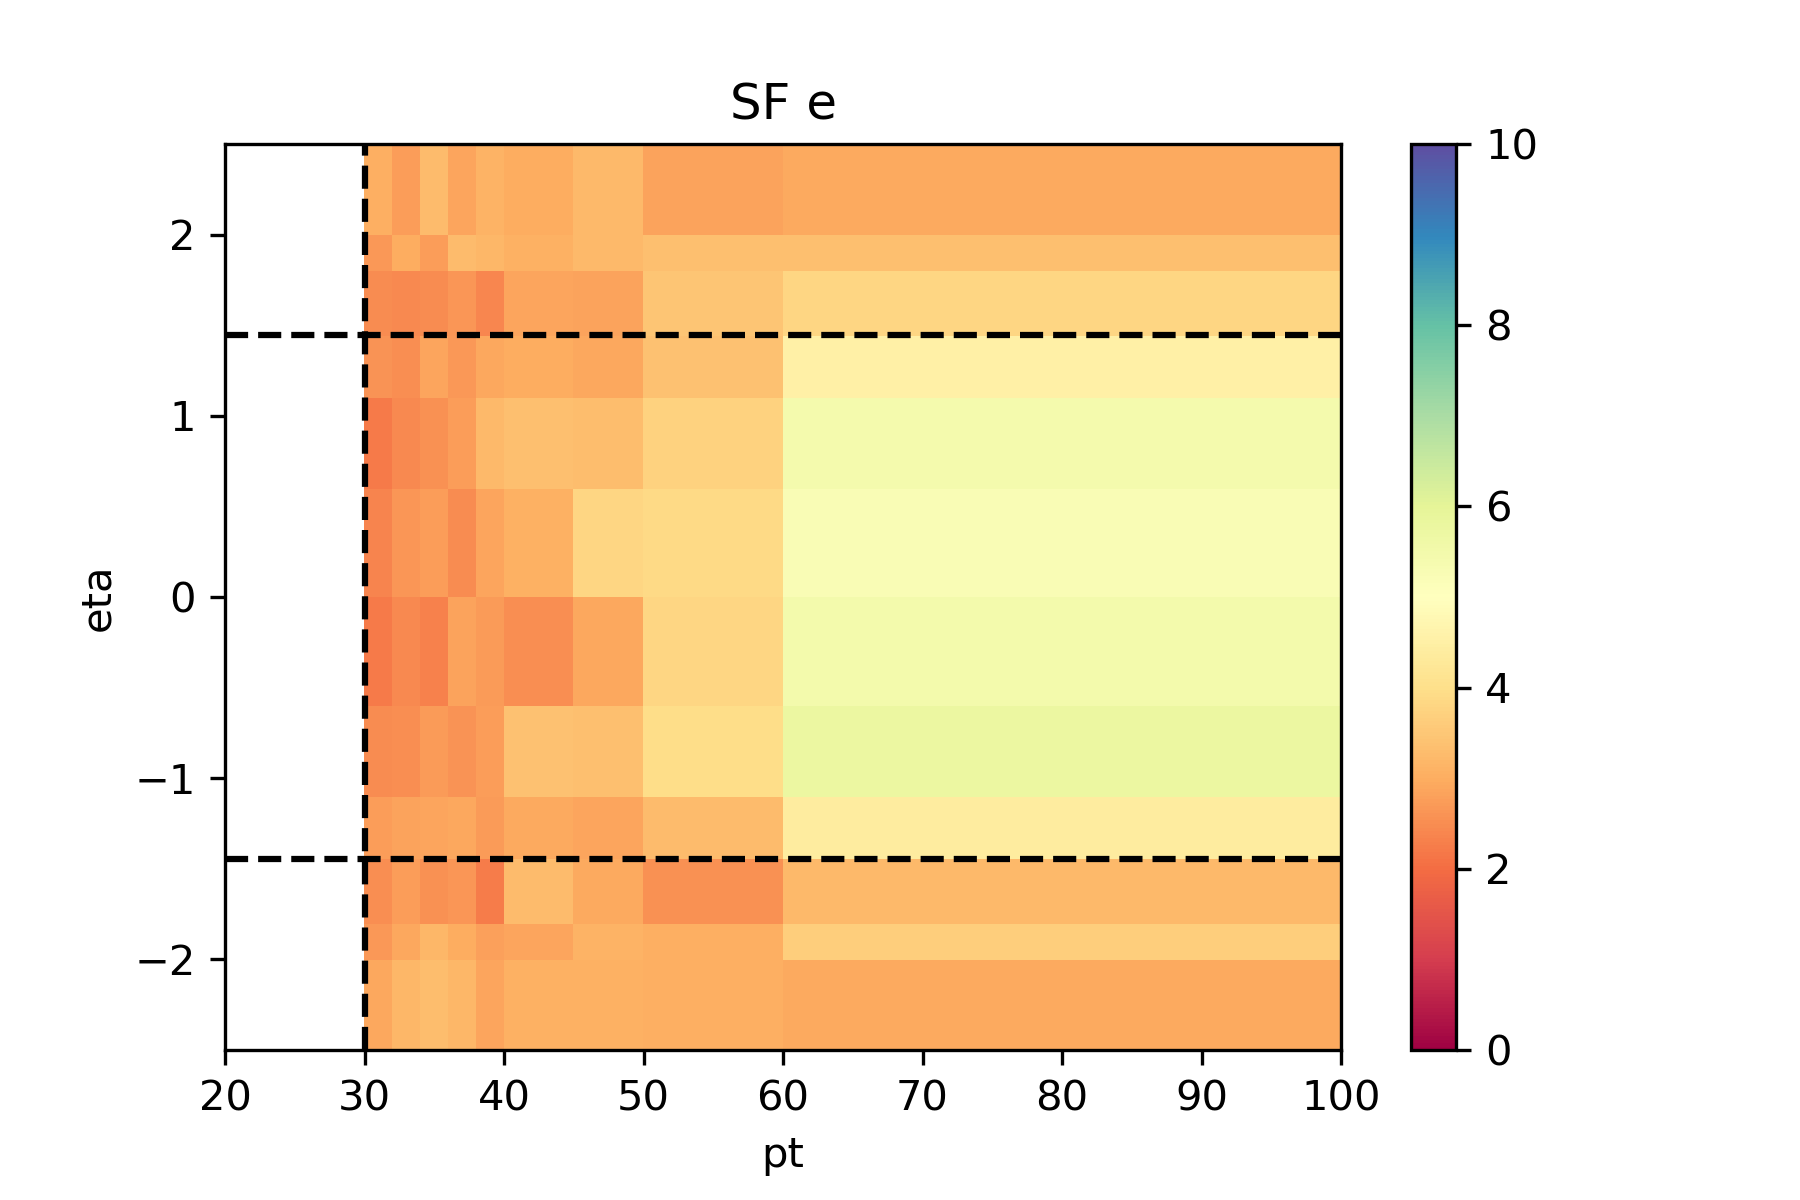
\includegraphics[width=0.49\textwidth]{chapters/Analysis/sectionBackground/figures/ljets_kinematics/123j1b/SF_e_2d.png}
    \caption{The $SF^{\rm \overline{iso} \to iso}$ measured in the lepton plus jet regions with $1\leq n_j<4$ and $n_\PQb\geq1$.}
    \label{fig:background:lh:123j1b_sf}
\end{figure}

\begin{figure}
    \centering
    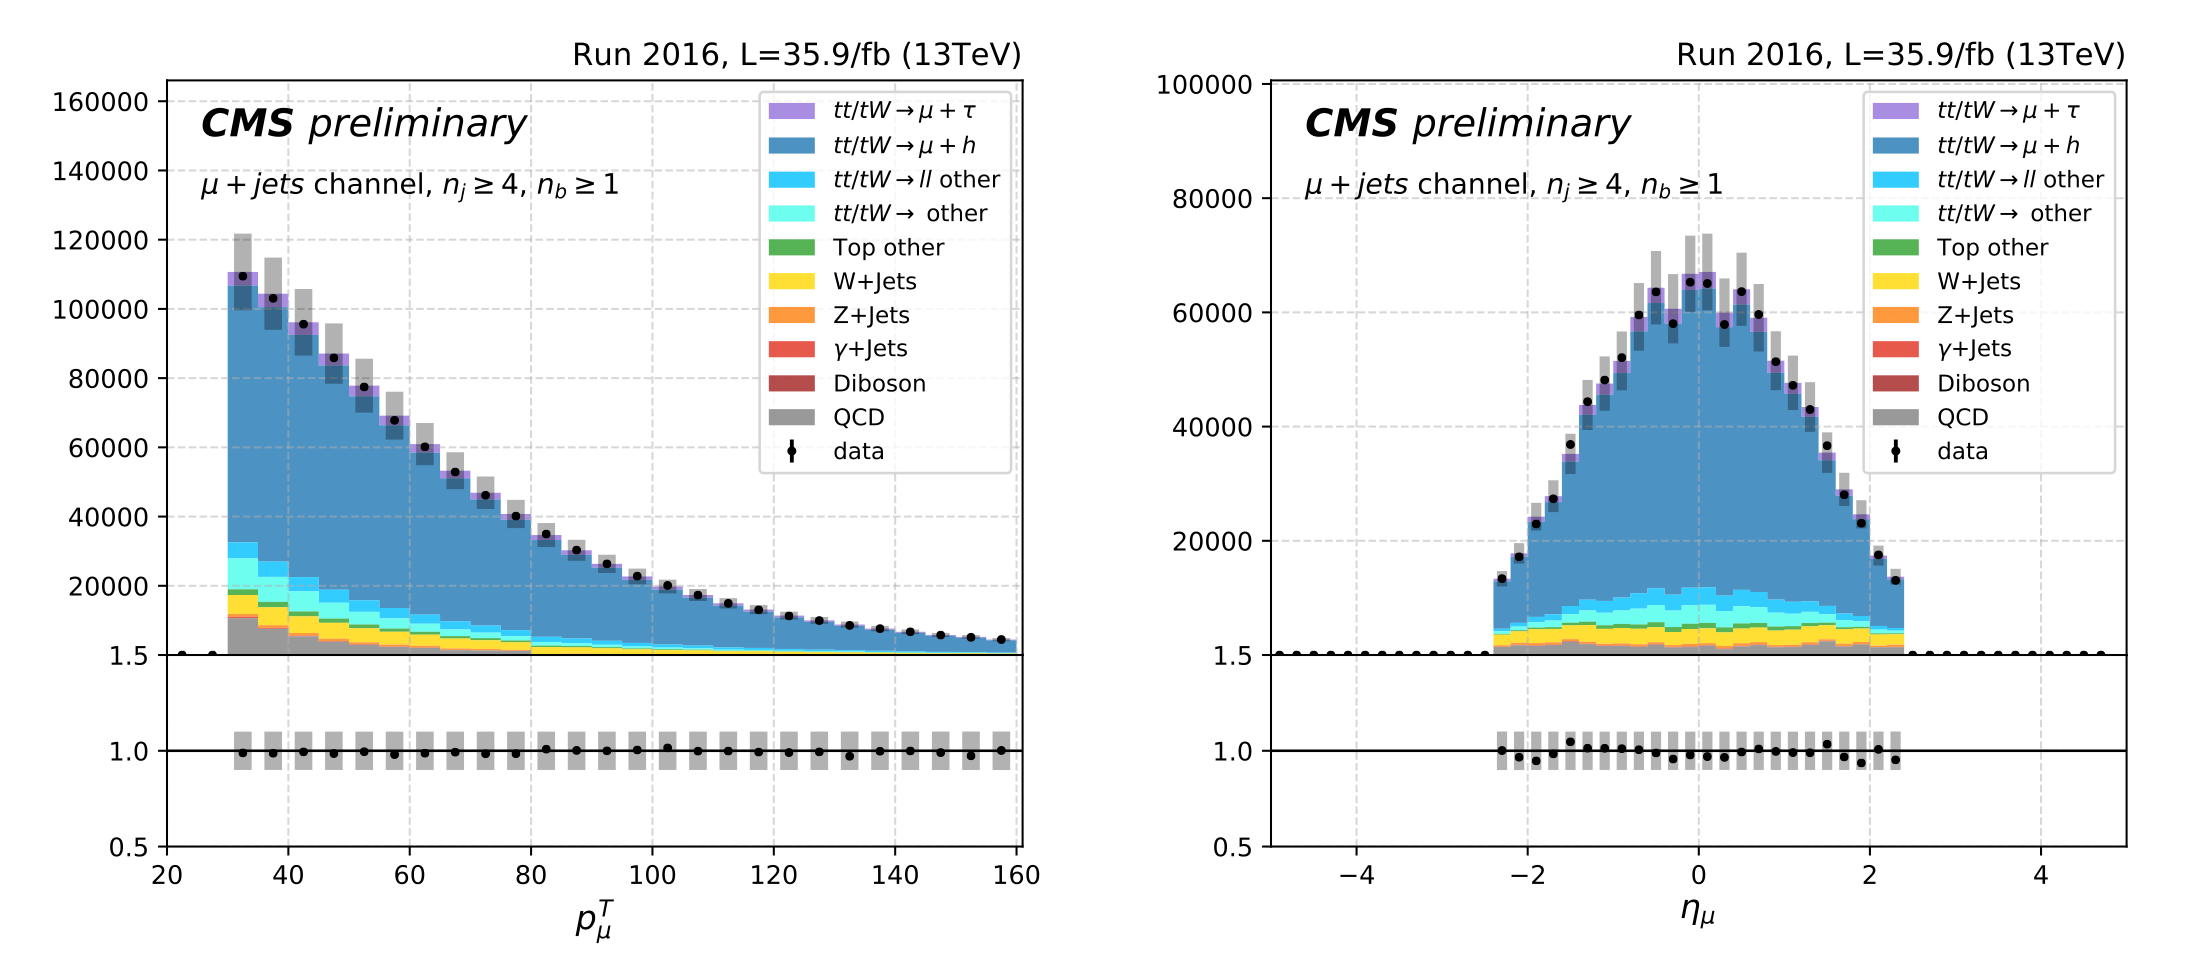
\includegraphics[width=0.9\textwidth]{chapters/Analysis/sectionBackground/figures/ljets_application/ddNorm_ddShape_mu4j.png}
    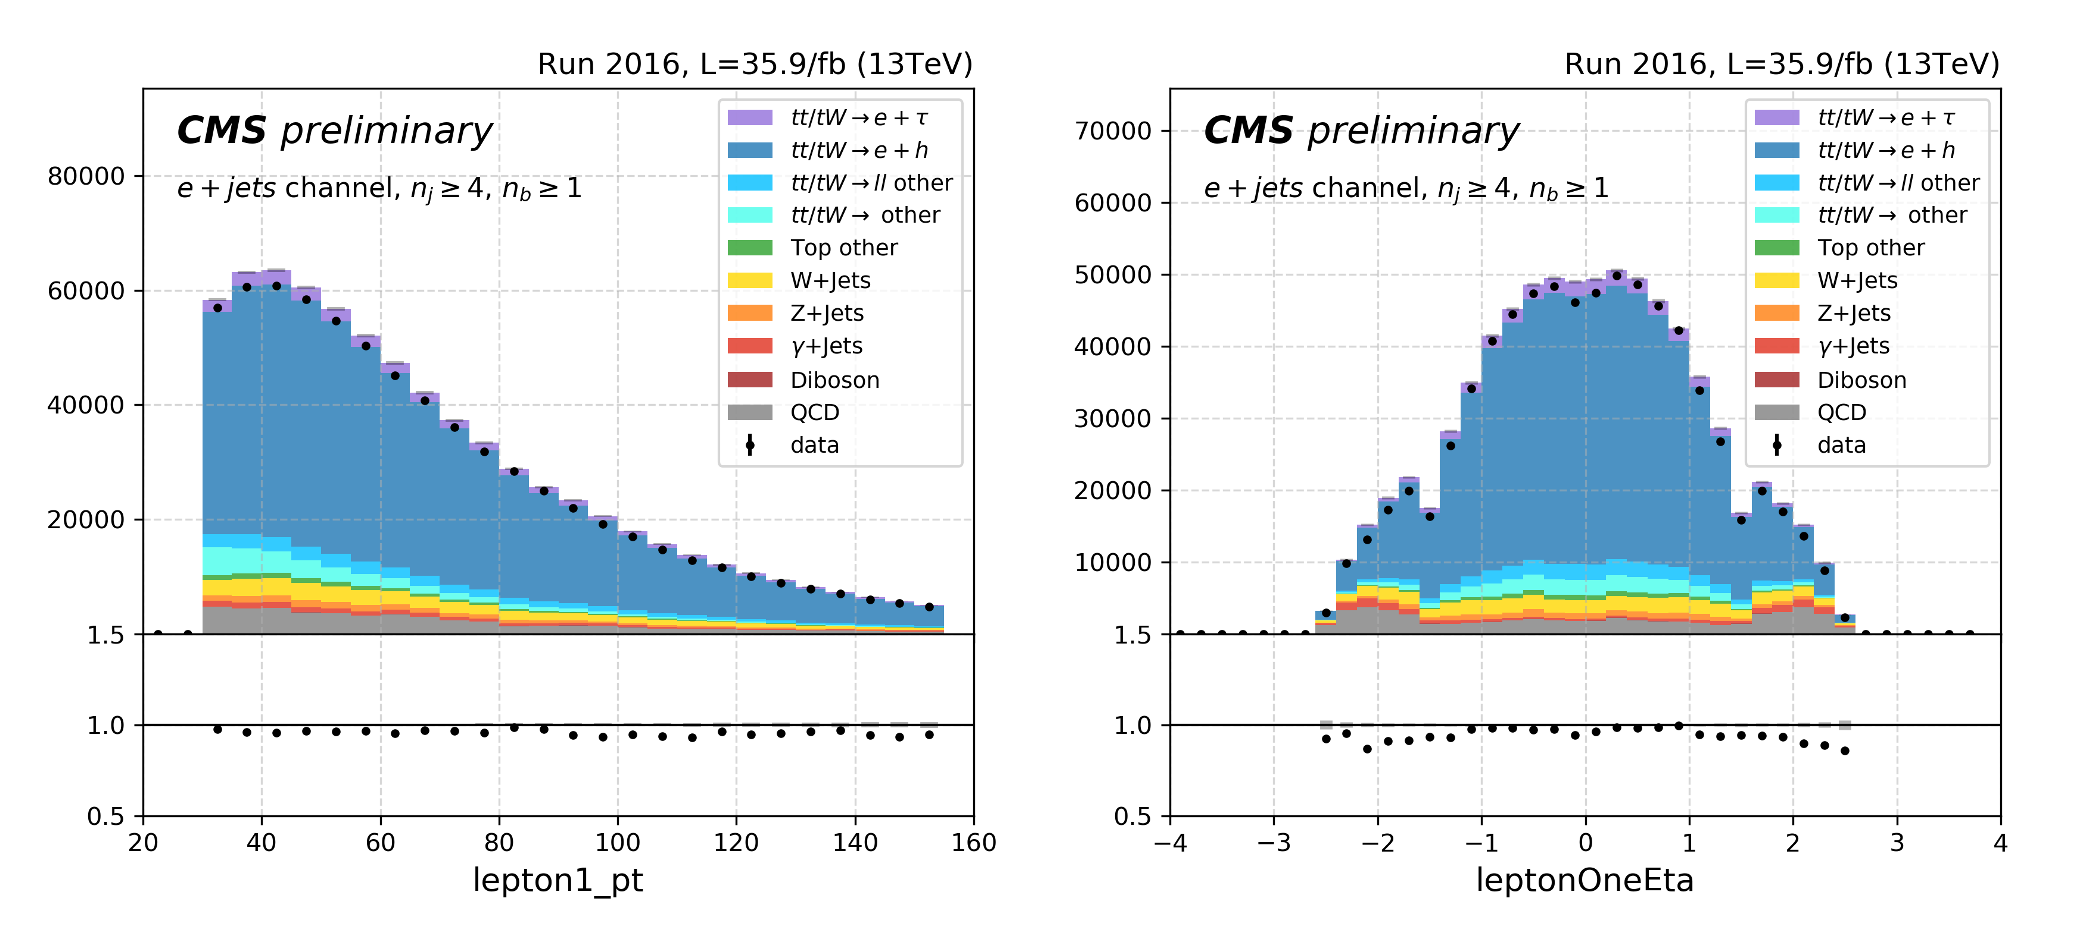
\includegraphics[width=0.9\textwidth]{chapters/Analysis/sectionBackground/figures/ljets_application/ddNorm_ddShape_e4j.png}
    \caption{Fully data-driven QCD estimation in \cmh and \ceh signal regions with $n_j\geq4$ and $n_\PQb\geq1$ based on the anti-isolation region with $SF^{\rm \overline{iso} \to iso}$.}
    \label{fig:background:lh:application_ddNorm_ddShape}
\end{figure}




Applying the measured $SF^{\rm \overline{iso} \to iso}$ in the signal region (\ceh and \cmh channels with $n_j\geq4$ and $n_\PQb\geq1$), the result QCD estimations obtained are shown in Figure~\ref{fig:background:lh:application_ddNorm_ddShape}. It is observed that the QCD estimation in the \cmh channel is reasonable, while that in the \ceh channel is over-estimated. The isolated and anti-isolated regions of \ceh and \cmh channels with $n_j\geq4$ and $n_\PQb\geq1$ are shown in Figure~\ref{fig:background:lh:4j1b}, where the left and right two columns are for the \cmh channel and \ceh channel, respectively. Comparing the data-simulation difference in the isolated and anti-isolated regions, their shapes do demonstrate similarities. The over-estimation in the \ceh channel could come from the normalization of $SF^{\rm \overline{iso} \to iso}$. In Figure~\ref{fig:background:lh:4j1b}, the QCD estimation from the \HT-binned QCD simulated  datasets is shown as red lines, which gives a decent estimation to the QCD normalization. If scale the anti-isolated region with the normalization of simulated dataset instead of the $SF^{\rm \overline{iso} \to iso}$, one gets a QCD estimation with data-driven shape and simulation-based normalization, shown in Figure~\ref{fig:app:QCD:application_SFNorm_ddShape}.

\begin{figure}
    \centering
    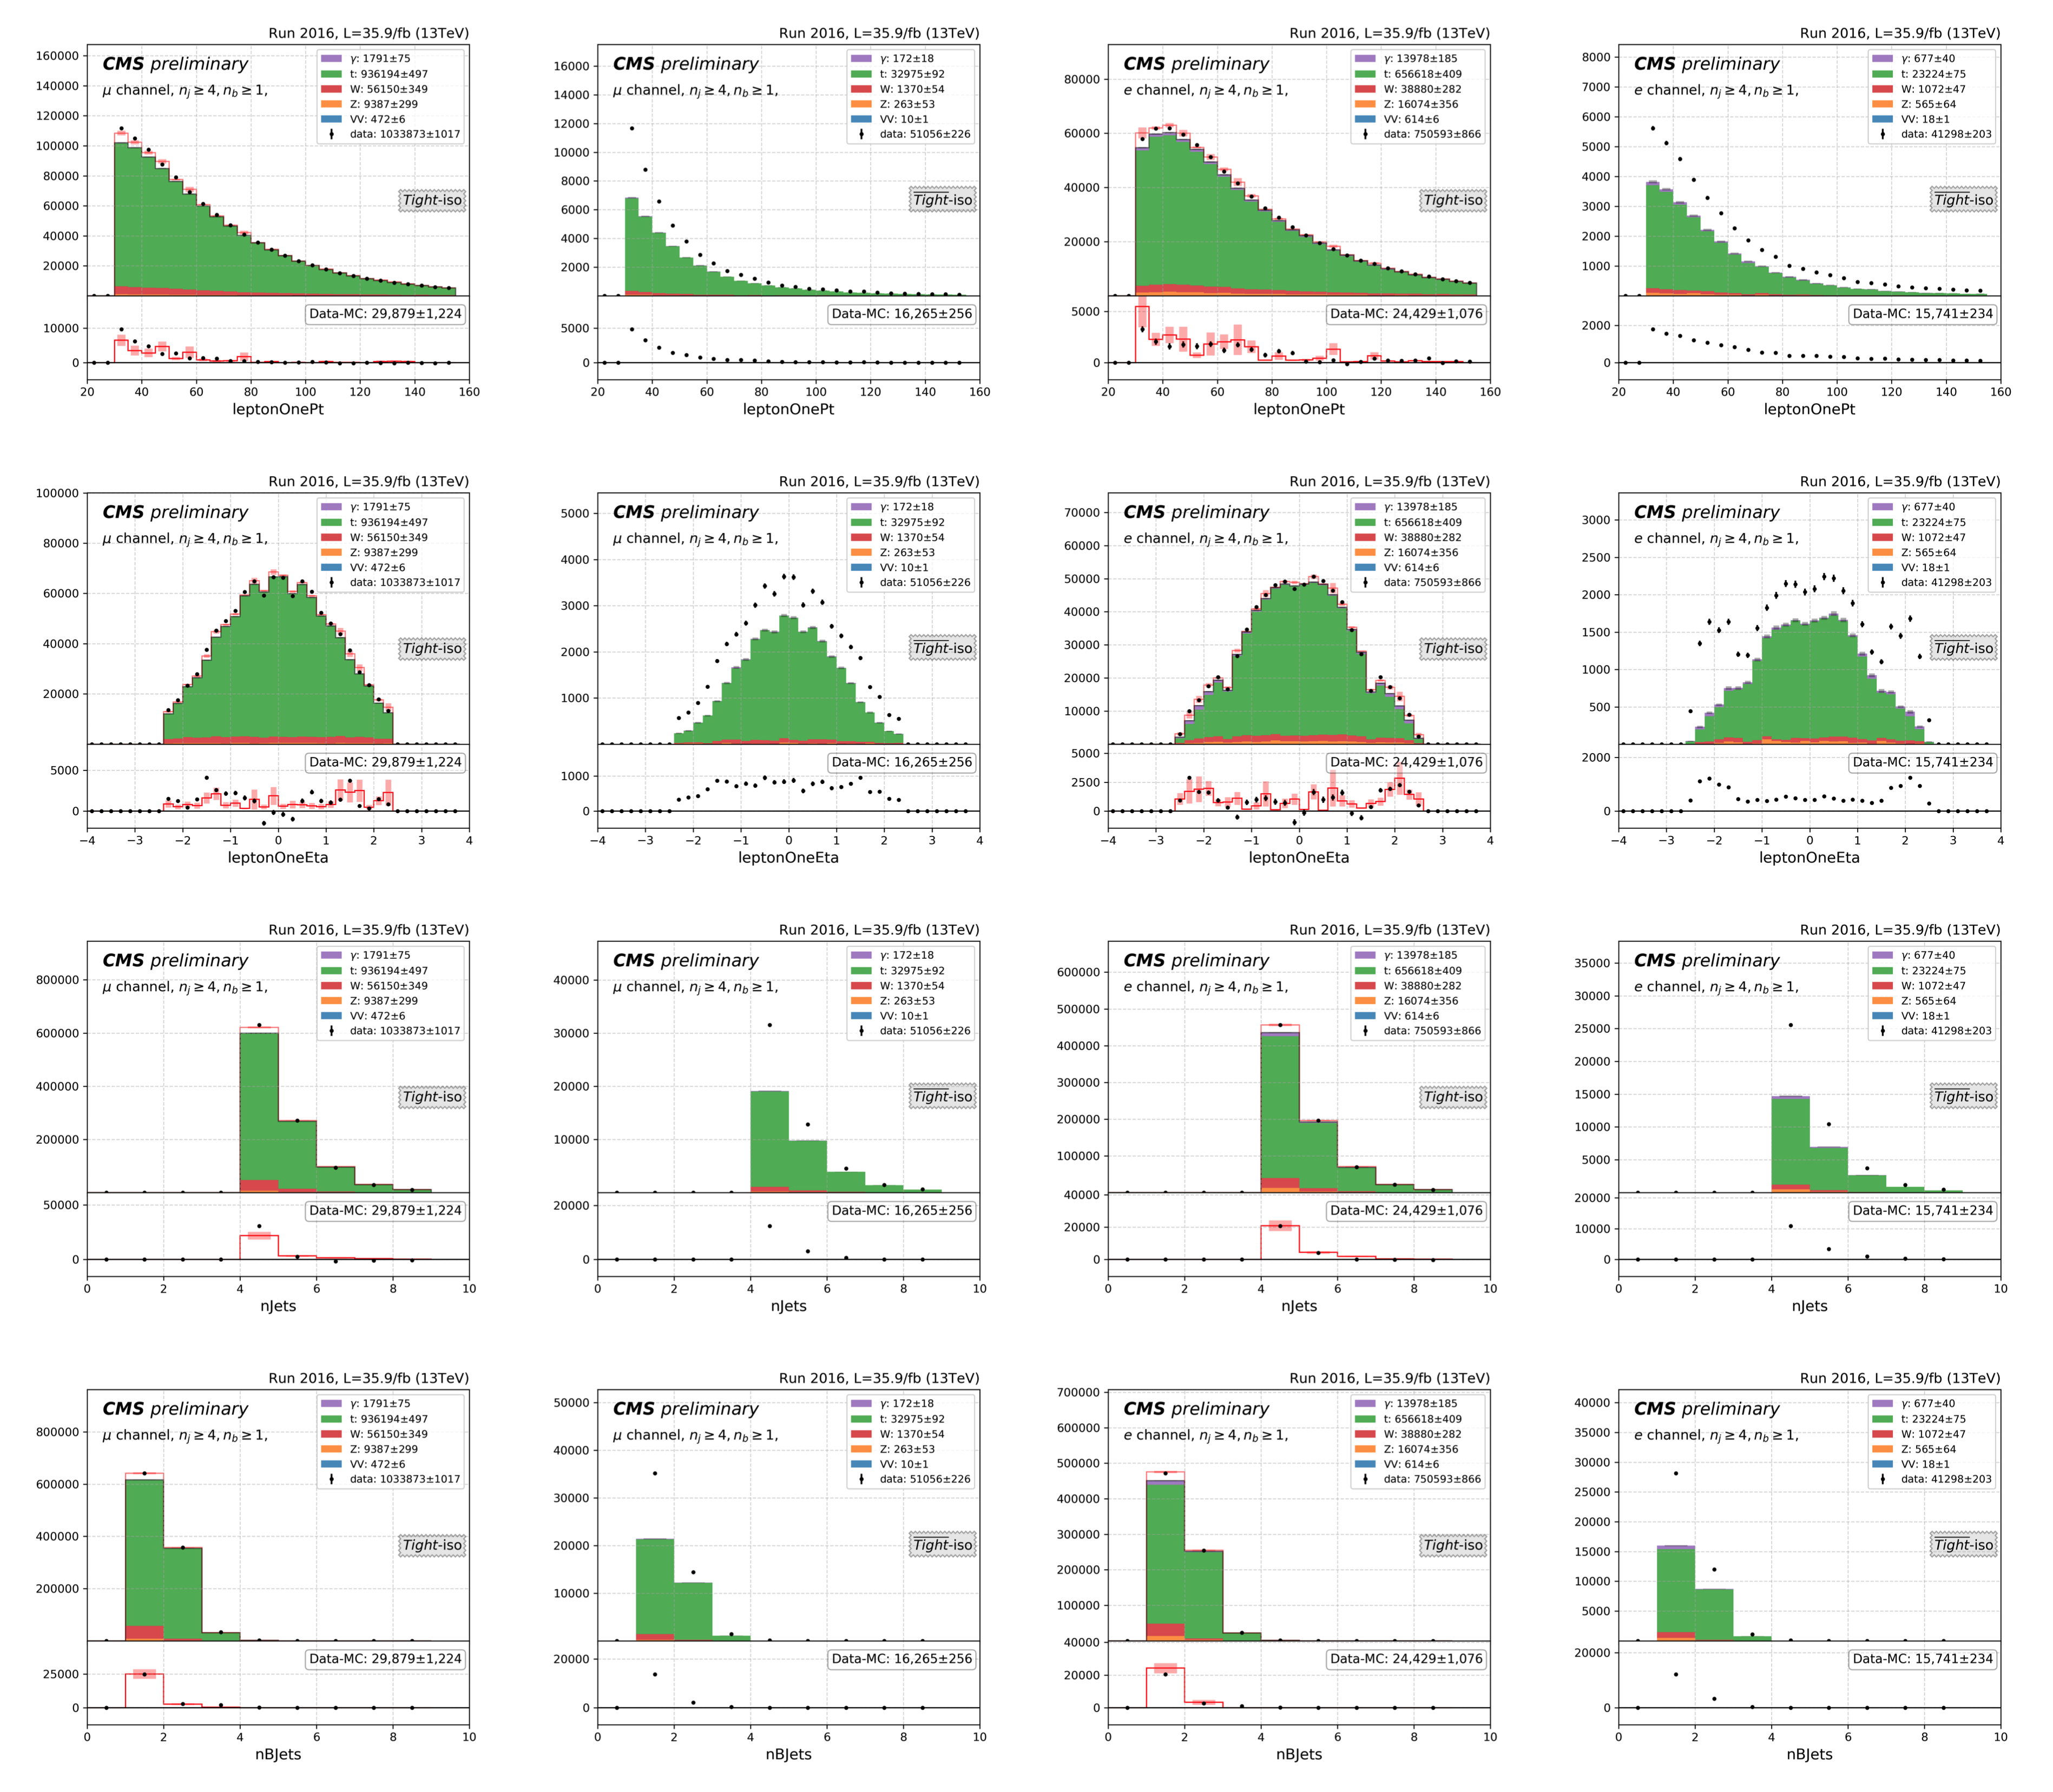
\includegraphics[width=0.99\textwidth]{chapters/Analysis/sectionBackground/figures/ljets_kinematics/4j1b.png}
    \caption{The isolated and anti-isolated regions of \ceh and \cmh channels with $n_j\geq4$ and $n_\PQb\geq1$. The left and right two columns are for the \cmh channel and \ceh channel, respectively}
    \label{fig:background:lh:4j1b}
\end{figure}
\begin{figure}
    \centering
    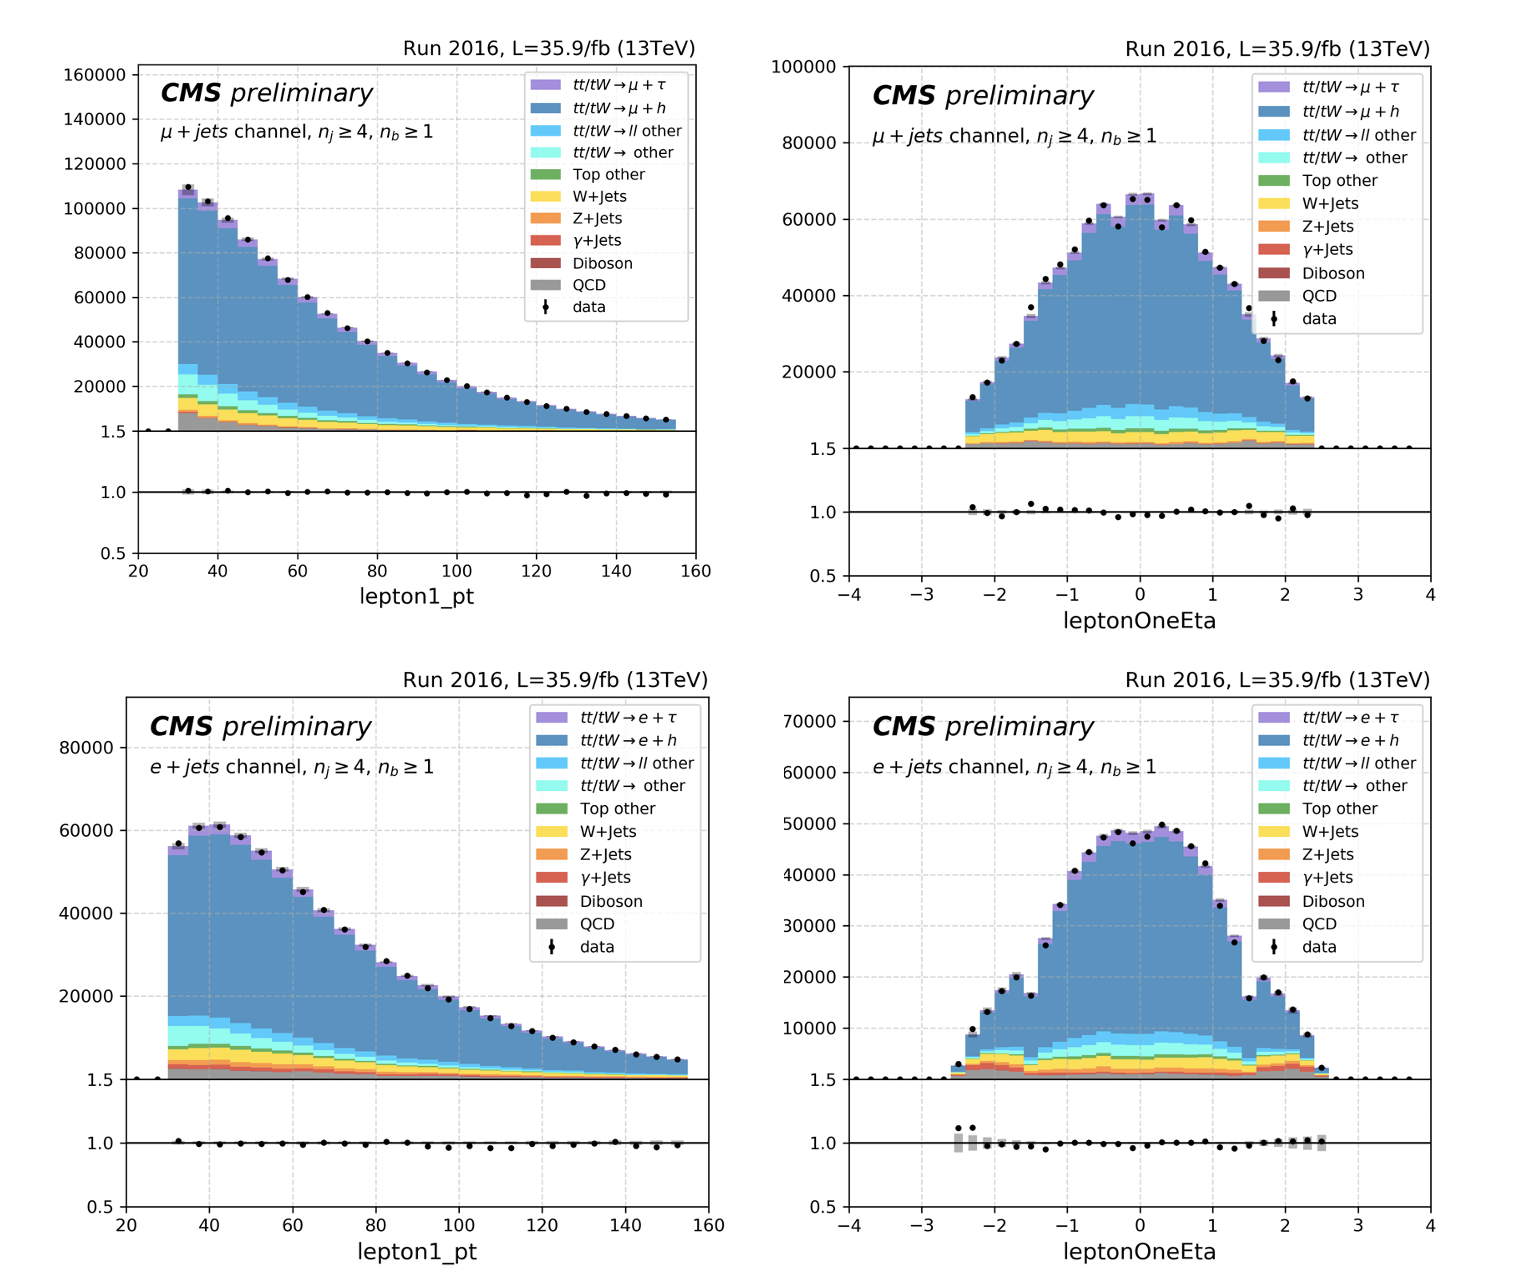
\includegraphics[width=0.99\textwidth]{chapters/Analysis/sectionBackground/figures/ljets_application/mcNorm_ddShape.png}
    \caption{The QCD estimation in \cmh and \ceh signal regions with $n_j\geq4$ and $n_\PQb\geq1$ based on data-driven shape and simulation-based normalization.}
    \label{fig:app:QCD:application_SFNorm_ddShape}
\end{figure}


For the counting analysis, the simulation-based normalization obtained from the HT-binned QCD simulated datasets is used. The statistical uncertainty of the simulation is about 4\%. To be conservative, a 30\% uncertainty is assigned to the QCD estimation. For the shape analysis, the shape of estimated QCD is from the anti-isolated region while the normalization is treated as a free parameters.








% \begin{figure}
%     \centering
%     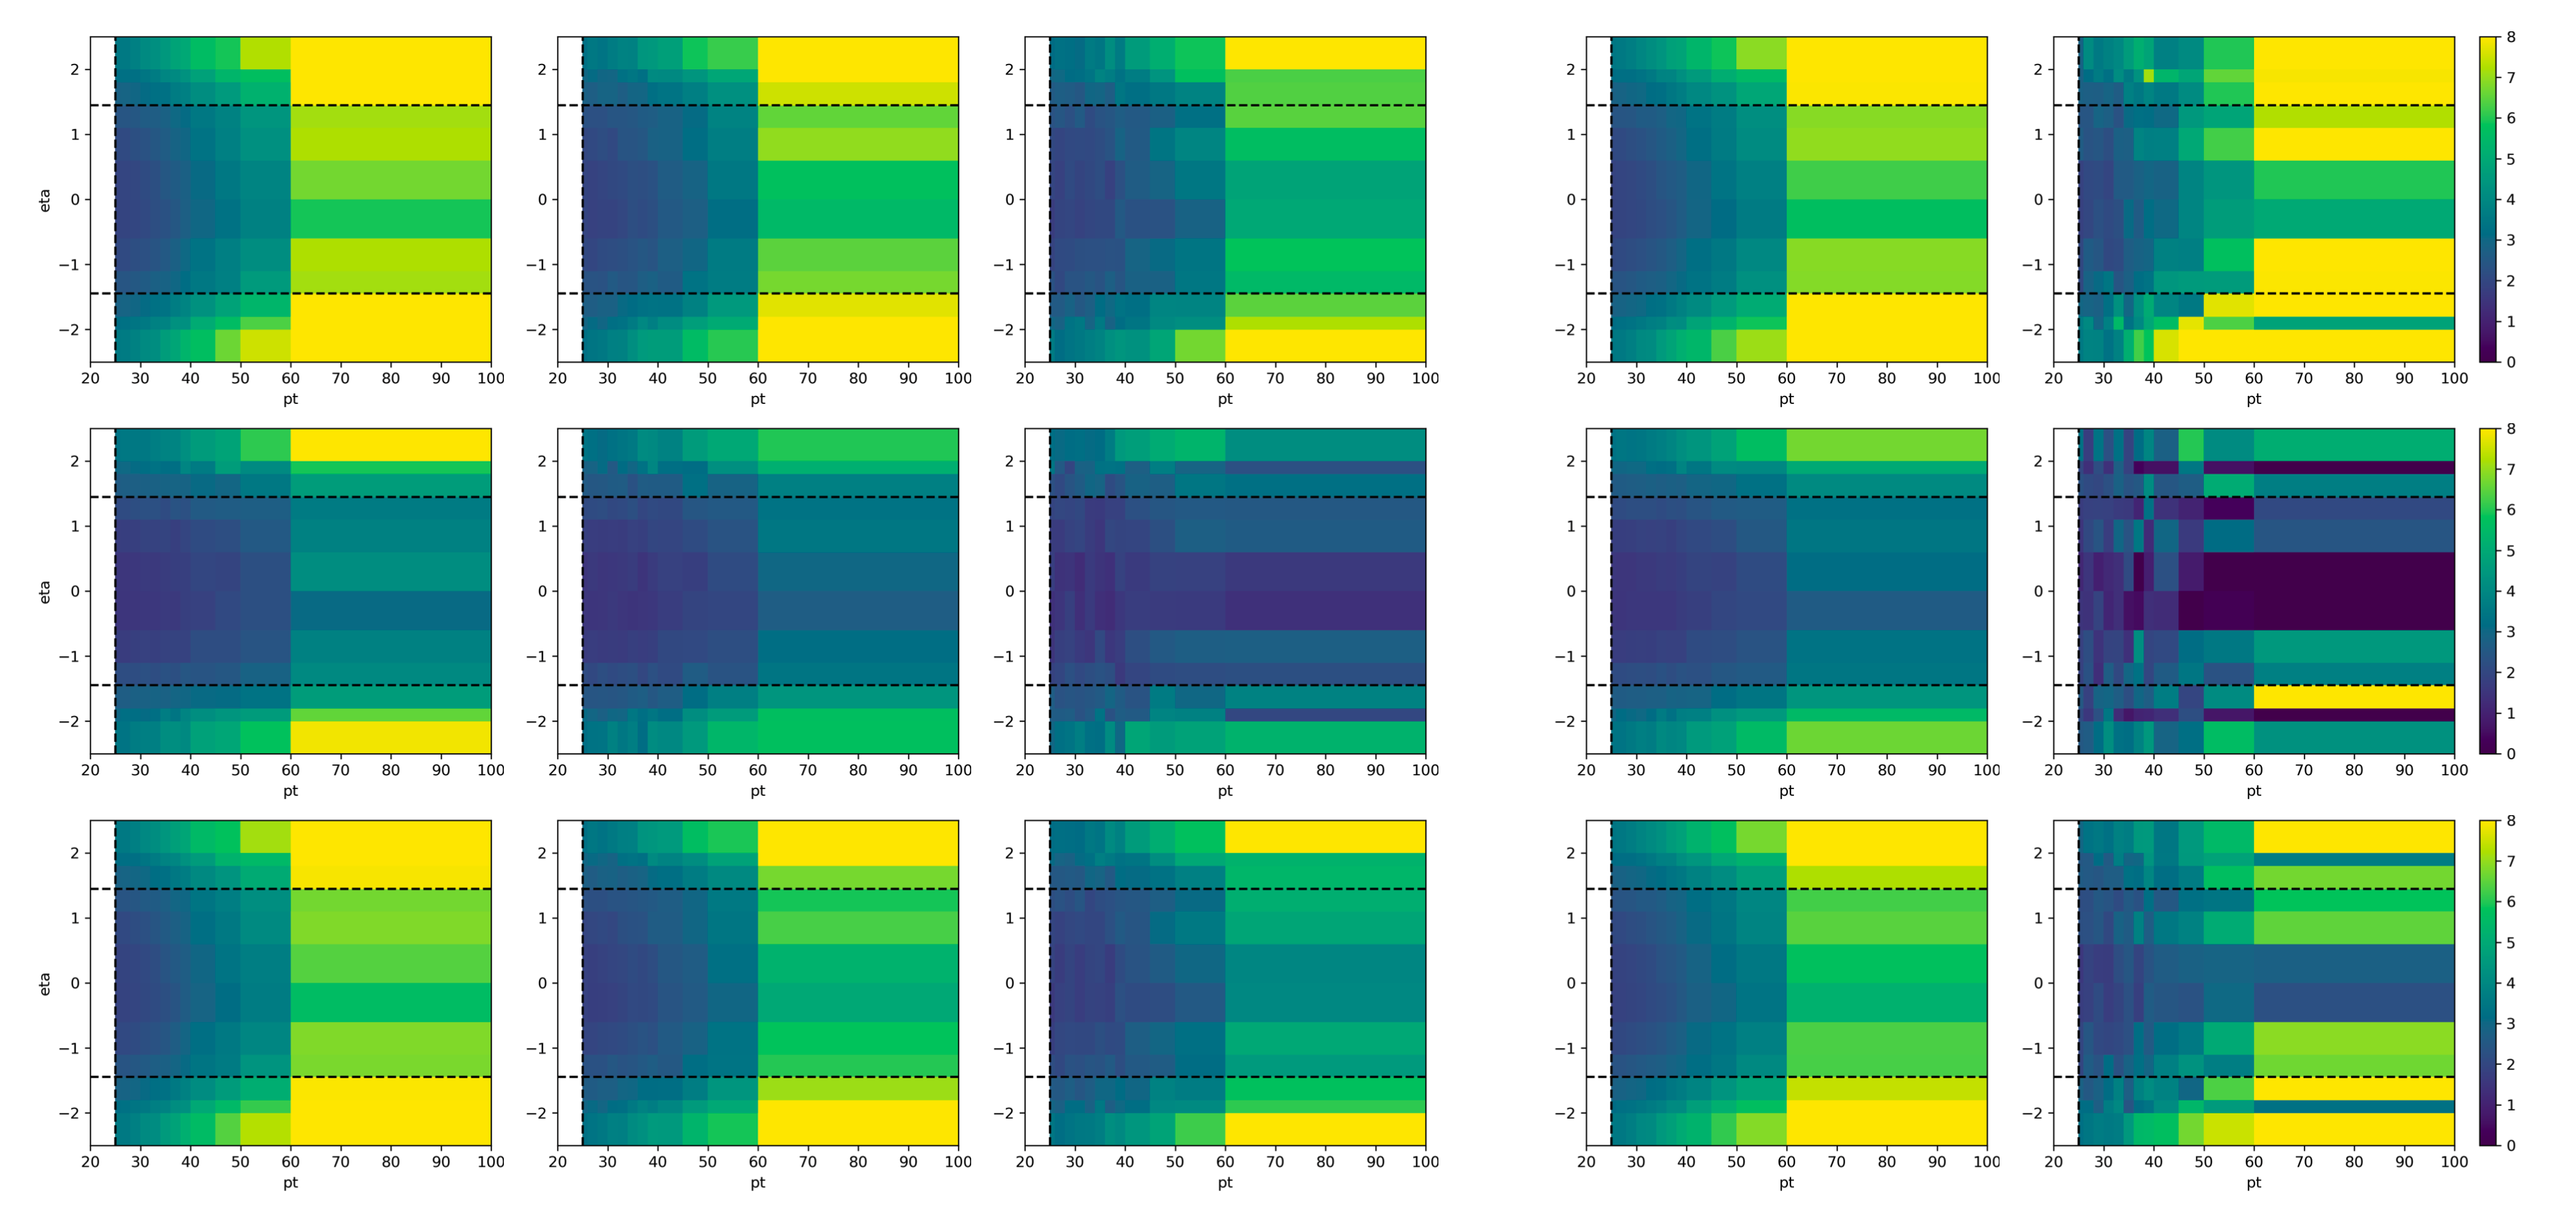
\includegraphics[width=0.99\textwidth]{chapters/Analysis/sectionBackground/figures/ljets_kinematics/sf_mu4j.png}
%     \caption{iso-to-antiiso SF in the $\mu$+jet all regions.}
%     \label{fig:background:lh:allsf}
% \end{figure}

% \begin{figure}
%     \centering
%     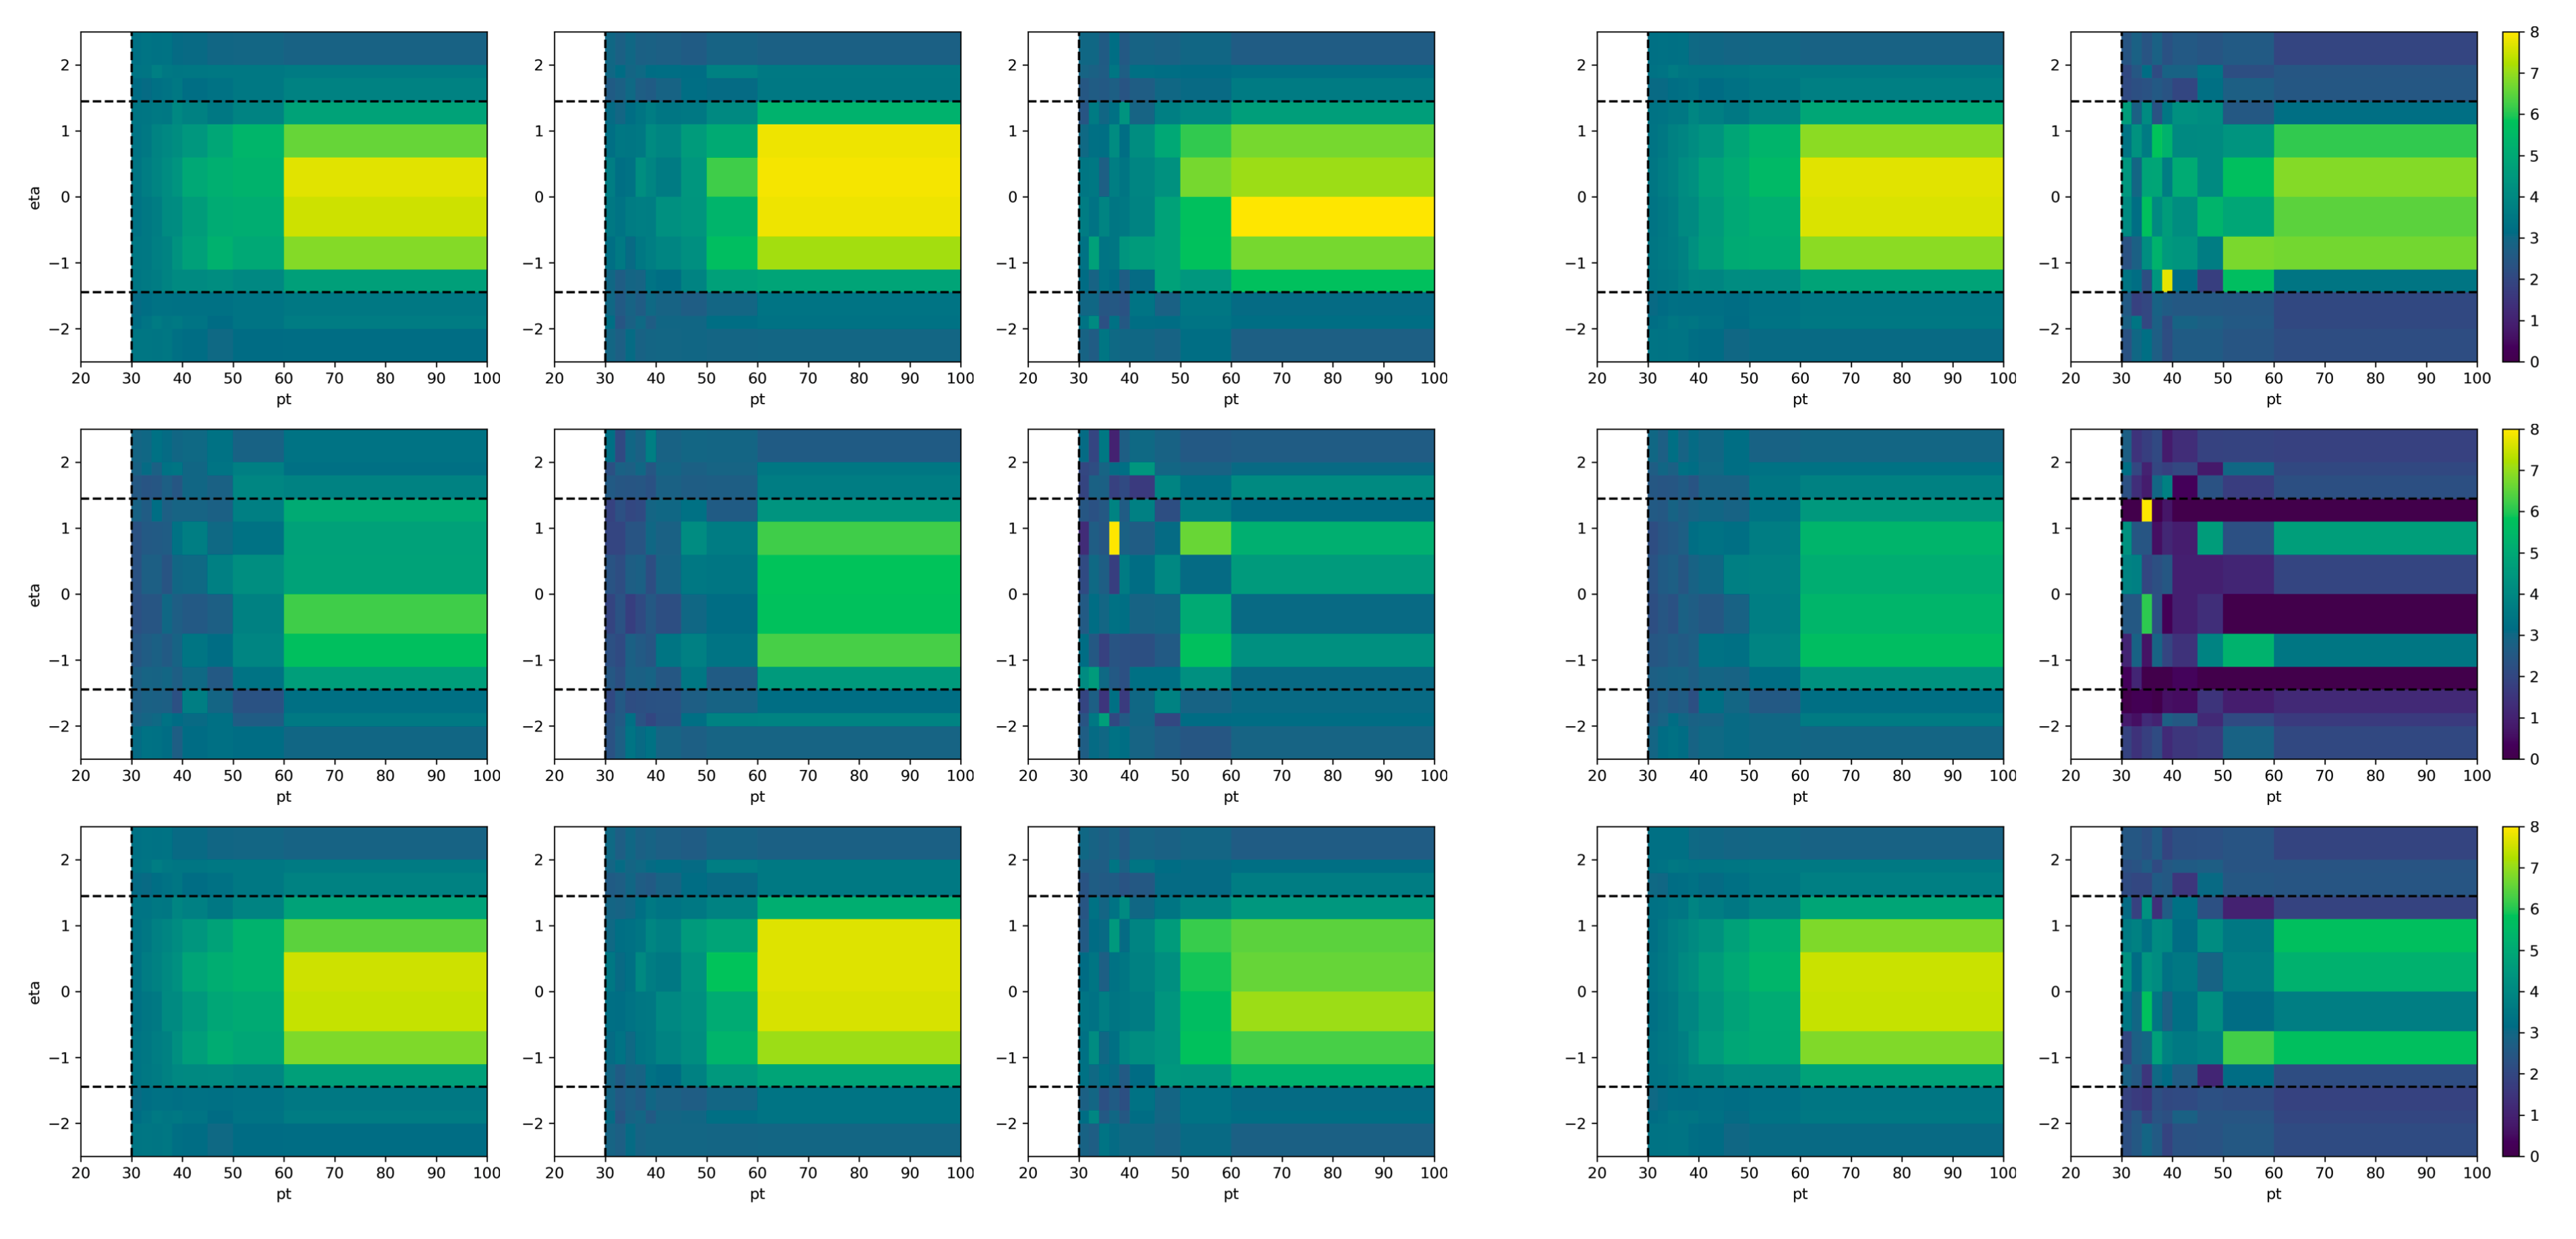
\includegraphics[width=0.99\textwidth]{chapters/Analysis/sectionBackground/figures/ljets_kinematics/sf_e4j.png}
%     \caption{iso-to-antiiso SF in the $e$+jet all regions.}
%     \label{fig:background:lh:allsf}
% \end{figure}


% \begin{figure}
%     \centering
%     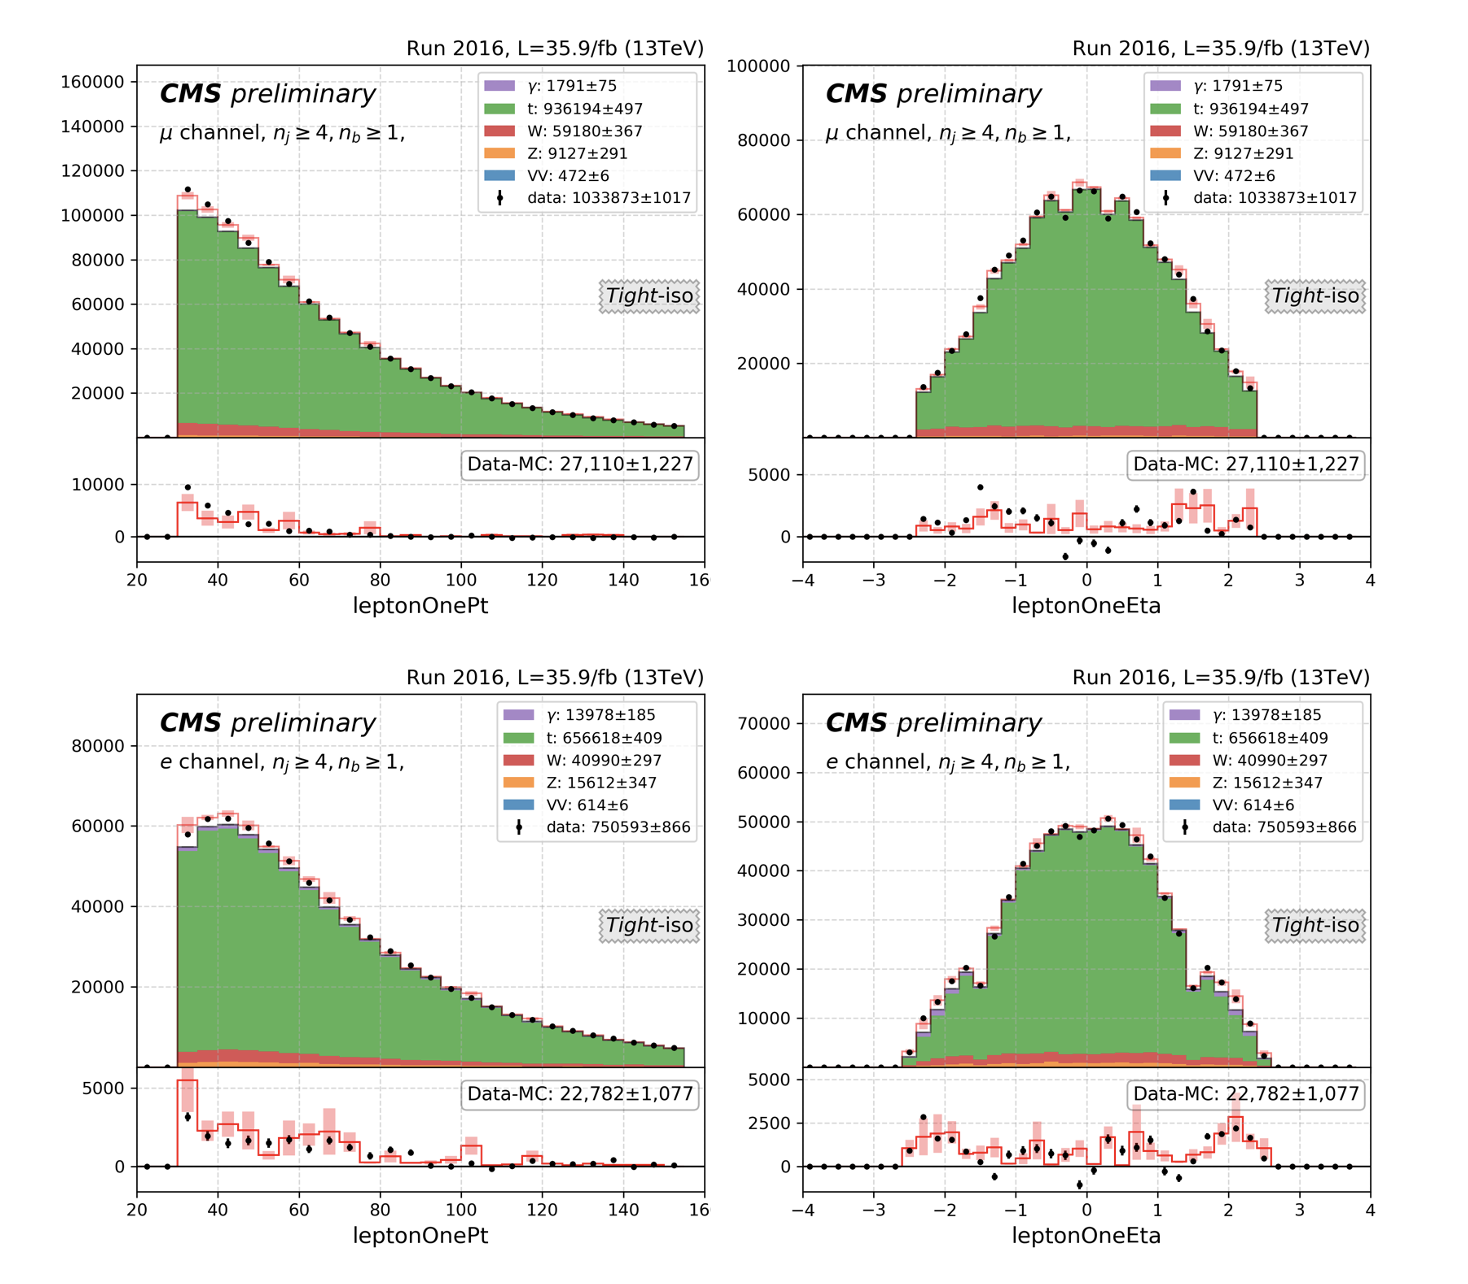
\includegraphics[width=0.99\textwidth]{chapters/Analysis/sectionBackground/figures/ljets_application/mcNorm_mcShape.png}
%     \caption{Fully MC-based QCD estimation}
%     \label{fig:app:QCD:application_mc}
% \end{figure}


